\documentclass[twoside]{book}

% Packages required by doxygen
\usepackage{fixltx2e}
\usepackage{calc}
\usepackage{doxygen}
\usepackage[export]{adjustbox} % also loads graphicx
\usepackage{graphicx}
\usepackage[utf8]{inputenc}
\usepackage{makeidx}
\usepackage{multicol}
\usepackage{multirow}
\PassOptionsToPackage{warn}{textcomp}
\usepackage{textcomp}
\usepackage[nointegrals]{wasysym}
\usepackage[table]{xcolor}

% Font selection
\usepackage[T1]{fontenc}
\usepackage[scaled=.90]{helvet}
\usepackage{courier}
\usepackage{amssymb}
\usepackage{sectsty}
\renewcommand{\familydefault}{\sfdefault}
\allsectionsfont{%
  \fontseries{bc}\selectfont%
  \color{darkgray}%
}
\renewcommand{\DoxyLabelFont}{%
  \fontseries{bc}\selectfont%
  \color{darkgray}%
}
\newcommand{\+}{\discretionary{\mbox{\scriptsize$\hookleftarrow$}}{}{}}

% Page & text layout
\usepackage{geometry}
\geometry{%
  a4paper,%
  top=2.5cm,%
  bottom=2.5cm,%
  left=2.5cm,%
  right=2.5cm%
}
\tolerance=750
\hfuzz=15pt
\hbadness=750
\setlength{\emergencystretch}{15pt}
\setlength{\parindent}{0cm}
\setlength{\parskip}{0.2cm}
\makeatletter
\renewcommand{\paragraph}{%
  \@startsection{paragraph}{4}{0ex}{-1.0ex}{1.0ex}{%
    \normalfont\normalsize\bfseries\SS@parafont%
  }%
}
\renewcommand{\subparagraph}{%
  \@startsection{subparagraph}{5}{0ex}{-1.0ex}{1.0ex}{%
    \normalfont\normalsize\bfseries\SS@subparafont%
  }%
}
\makeatother

% Headers & footers
\usepackage{fancyhdr}
\pagestyle{fancyplain}
\fancyhead[LE]{\fancyplain{}{\bfseries\thepage}}
\fancyhead[CE]{\fancyplain{}{}}
\fancyhead[RE]{\fancyplain{}{\bfseries\leftmark}}
\fancyhead[LO]{\fancyplain{}{\bfseries\rightmark}}
\fancyhead[CO]{\fancyplain{}{}}
\fancyhead[RO]{\fancyplain{}{\bfseries\thepage}}
\fancyfoot[LE]{\fancyplain{}{}}
\fancyfoot[CE]{\fancyplain{}{}}
\fancyfoot[RE]{\fancyplain{}{\bfseries\scriptsize Generated on Thu Sep 29 2016 00\+:19\+:10 for My Project by Doxygen }}
\fancyfoot[LO]{\fancyplain{}{\bfseries\scriptsize Generated on Thu Sep 29 2016 00\+:19\+:10 for My Project by Doxygen }}
\fancyfoot[CO]{\fancyplain{}{}}
\fancyfoot[RO]{\fancyplain{}{}}
\renewcommand{\footrulewidth}{0.4pt}
\renewcommand{\chaptermark}[1]{%
  \markboth{#1}{}%
}
\renewcommand{\sectionmark}[1]{%
  \markright{\thesection\ #1}%
}

% Indices & bibliography
\usepackage{natbib}
\usepackage[titles]{tocloft}
\setcounter{tocdepth}{3}
\setcounter{secnumdepth}{5}
\makeindex

% Hyperlinks (required, but should be loaded last)
\usepackage{ifpdf}
\ifpdf
  \usepackage[pdftex,pagebackref=true]{hyperref}
\else
  \usepackage[ps2pdf,pagebackref=true]{hyperref}
\fi
\hypersetup{%
  colorlinks=true,%
  linkcolor=blue,%
  citecolor=blue,%
  unicode%
}

% Custom commands
\newcommand{\clearemptydoublepage}{%
  \newpage{\pagestyle{empty}\cleardoublepage}%
}


%===== C O N T E N T S =====

\begin{document}

% Titlepage & ToC
\hypersetup{pageanchor=false,
             bookmarks=true,
             bookmarksnumbered=true,
             pdfencoding=unicode
            }
\pagenumbering{roman}
\begin{titlepage}
\vspace*{7cm}
\begin{center}%
{\Large My Project }\\
\vspace*{1cm}
{\large Generated by Doxygen 1.8.10}\\
\vspace*{0.5cm}
{\small Thu Sep 29 2016 00:19:10}\\
\end{center}
\end{titlepage}
\clearemptydoublepage
\tableofcontents
\clearemptydoublepage
\pagenumbering{arabic}
\hypersetup{pageanchor=true}

%--- Begin generated contents ---
\chapter{Gantt documentation}
\label{index}\hypertarget{index}{}\hypertarget{index_intro_sec}{}\section{Introduction}\label{index_intro_sec}
Basic functionality\+:

\hyperlink{class_main_window_a02076de46e6810174817ebfc6ddd2be5}{Main\+Window\+::reset()} will clear or reset everything. \hyperlink{class_main_window_a580a35d29abc0a0c82edf183e7f87b74}{Main\+Window\+::open\+C\+S\+V()} or \hyperlink{class_main_window_a23e9c749c8f0e5119317ea6484b9476f}{Main\+Window\+::open\+G\+D\+X()} will add flows and tasks with \hyperlink{class_main_window_a2920d5c6c64925cb5f87c7fdac3f54b0}{Main\+Window\+::add\+Task()} and \hyperlink{class_main_window_a645f1cd085c2636dc4eccb320455a6f4}{Main\+Window\+::add\+Flow()}. \hyperlink{class_main_window_a0b3d1510d0e0ed665daa74d6823e00d6}{Main\+Window\+::create\+Representation} will \char`\"{}bake\char`\"{} all tasks and flows and generate the scene.\hypertarget{index_install_sec}{}\section{Installation}\label{index_install_sec}
To cross compile on unix for any platform\+: \href{http://stackoverflow.com/questions/14170590/building-qt-5-on-linux-for-windows/14170591#14170591}{\tt http\+://stackoverflow.\+com/questions/14170590/building-\/qt-\/5-\/on-\/linux-\/for-\/windows/14170591\#14170591}


\begin{DoxyEnumerate}
\item add mxe to P\+A\+T\+H\+:
\begin{DoxyCode}
export PATH=$PATH:<mxe install location>/usr/bin 
\end{DoxyCode}

\item to compile for Windows, run
\begin{DoxyCode}
i686-w64-mingw32.static-qmake-qt5 
\end{DoxyCode}

\item run
\begin{DoxyCode}
make 
\end{DoxyCode}

\end{DoxyEnumerate}

\begin{DoxyAuthor}{Author}
Julius Naeumann, \href{mailto:julius.naeumann@gmail.com}{\tt julius.\+naeumann@gmail.\+com} 
\end{DoxyAuthor}
\begin{DoxyDate}{Date}
August 2016 
\end{DoxyDate}

\chapter{Namespace Index}
\section{Namespace List}
Here is a list of all documented namespaces with brief descriptions\+:\begin{DoxyCompactList}
\item\contentsline{section}{\hyperlink{namespace_ui}{Ui} \\*\hyperlink{namespace_ui}{Ui} namespace, containing the Main\+View and \hyperlink{class_ui_1_1_wizard}{Wizard} classes }{\pageref{namespace_ui}}{}
\end{DoxyCompactList}

\chapter{Hierarchical Index}
\section{Class Hierarchy}
This inheritance list is sorted roughly, but not completely, alphabetically\+:\begin{DoxyCompactList}
\item \contentsline{section}{Flow}{\pageref{struct_flow}}{}
\item Q\+Graphics\+Line\+Item\begin{DoxyCompactList}
\item \contentsline{section}{Gantt\+Line}{\pageref{class_gantt_line}}{}
\end{DoxyCompactList}
\item Q\+Graphics\+Polygon\+Item\begin{DoxyCompactList}
\item \contentsline{section}{Gantt\+Flow}{\pageref{class_gantt_flow}}{}
\end{DoxyCompactList}
\item Q\+Graphics\+Rect\+Item\begin{DoxyCompactList}
\item \contentsline{section}{Gantt\+Rect}{\pageref{class_gantt_rect}}{}
\end{DoxyCompactList}
\item Q\+Graphics\+View\begin{DoxyCompactList}
\item \contentsline{section}{Gantt\+Graphics\+View}{\pageref{class_gantt_graphics_view}}{}
\end{DoxyCompactList}
\item Q\+Main\+Window\begin{DoxyCompactList}
\item \contentsline{section}{Main\+Window}{\pageref{class_main_window}}{}
\end{DoxyCompactList}
\item Q\+Object\begin{DoxyCompactList}
\item \contentsline{section}{Gantt\+Flow}{\pageref{class_gantt_flow}}{}
\item \contentsline{section}{Gantt\+Line}{\pageref{class_gantt_line}}{}
\item \contentsline{section}{Gantt\+Rect}{\pageref{class_gantt_rect}}{}
\end{DoxyCompactList}
\item \contentsline{section}{qt\+\_\+meta\+\_\+stringdata\+\_\+\+Gantt\+Flow\+\_\+t}{\pageref{structqt__meta__stringdata___gantt_flow__t}}{}
\item \contentsline{section}{qt\+\_\+meta\+\_\+stringdata\+\_\+\+Gantt\+Rect\+\_\+t}{\pageref{structqt__meta__stringdata___gantt_rect__t}}{}
\item \contentsline{section}{qt\+\_\+meta\+\_\+stringdata\+\_\+\+Main\+Window\+\_\+t}{\pageref{structqt__meta__stringdata___main_window__t}}{}
\item \contentsline{section}{qt\+\_\+meta\+\_\+stringdata\+\_\+\+Wizard\+\_\+t}{\pageref{structqt__meta__stringdata___wizard__t}}{}
\item Q\+Table\+Widget\+Item\begin{DoxyCompactList}
\item \contentsline{section}{Q\+Table\+Widget\+Number\+Item}{\pageref{class_q_table_widget_number_item}}{}
\end{DoxyCompactList}
\item Q\+Wizard\begin{DoxyCompactList}
\item \contentsline{section}{Wizard}{\pageref{class_wizard}}{}
\end{DoxyCompactList}
\item \contentsline{section}{Raw\+Flow}{\pageref{struct_raw_flow}}{}
\item \contentsline{section}{Raw\+Task}{\pageref{struct_raw_task}}{}
\item \contentsline{section}{Task}{\pageref{struct_task}}{}
\item \contentsline{section}{Ui\+\_\+\+Main\+Window}{\pageref{class_ui___main_window}}{}
\begin{DoxyCompactList}
\item \contentsline{section}{Ui\+:\+:Main\+Window}{\pageref{class_ui_1_1_main_window}}{}
\end{DoxyCompactList}
\item \contentsline{section}{Ui\+\_\+\+Wizard}{\pageref{class_ui___wizard}}{}
\begin{DoxyCompactList}
\item \contentsline{section}{Ui\+:\+:Wizard}{\pageref{class_ui_1_1_wizard}}{}
\end{DoxyCompactList}
\end{DoxyCompactList}

\chapter{Class Index}
\section{Class List}
Here are the classes, structs, unions and interfaces with brief descriptions\+:\begin{DoxyCompactList}
\item\contentsline{section}{\hyperlink{struct_flow}{Flow} \\*Representation of a flow }{\pageref{struct_flow}}{}
\item\contentsline{section}{\hyperlink{class_gantt_flow}{Gantt\+Flow} }{\pageref{class_gantt_flow}}{}
\item\contentsline{section}{\hyperlink{class_gantt_graphics_view}{Gantt\+Graphics\+View} }{\pageref{class_gantt_graphics_view}}{}
\item\contentsline{section}{\hyperlink{class_gantt_line}{Gantt\+Line} }{\pageref{class_gantt_line}}{}
\item\contentsline{section}{\hyperlink{class_gantt_rect}{Gantt\+Rect} }{\pageref{class_gantt_rect}}{}
\item\contentsline{section}{\hyperlink{class_main_window}{Main\+Window} \\*Class for the Main window }{\pageref{class_main_window}}{}
\item\contentsline{section}{\hyperlink{class_ui_1_1_main_window}{Ui\+::\+Main\+Window} }{\pageref{class_ui_1_1_main_window}}{}
\item\contentsline{section}{\hyperlink{structqt__meta__stringdata___gantt_flow__t}{qt\+\_\+meta\+\_\+stringdata\+\_\+\+Gantt\+Flow\+\_\+t} }{\pageref{structqt__meta__stringdata___gantt_flow__t}}{}
\item\contentsline{section}{\hyperlink{structqt__meta__stringdata___gantt_rect__t}{qt\+\_\+meta\+\_\+stringdata\+\_\+\+Gantt\+Rect\+\_\+t} }{\pageref{structqt__meta__stringdata___gantt_rect__t}}{}
\item\contentsline{section}{\hyperlink{structqt__meta__stringdata___main_window__t}{qt\+\_\+meta\+\_\+stringdata\+\_\+\+Main\+Window\+\_\+t} }{\pageref{structqt__meta__stringdata___main_window__t}}{}
\item\contentsline{section}{\hyperlink{structqt__meta__stringdata___wizard__t}{qt\+\_\+meta\+\_\+stringdata\+\_\+\+Wizard\+\_\+t} }{\pageref{structqt__meta__stringdata___wizard__t}}{}
\item\contentsline{section}{\hyperlink{class_q_table_widget_number_item}{Q\+Table\+Widget\+Number\+Item} }{\pageref{class_q_table_widget_number_item}}{}
\item\contentsline{section}{\hyperlink{struct_raw_flow}{Raw\+Flow} }{\pageref{struct_raw_flow}}{}
\item\contentsline{section}{\hyperlink{struct_raw_task}{Raw\+Task} }{\pageref{struct_raw_task}}{}
\item\contentsline{section}{\hyperlink{struct_task}{Task} \\*Representation of a task }{\pageref{struct_task}}{}
\item\contentsline{section}{\hyperlink{class_ui___main_window}{Ui\+\_\+\+Main\+Window} }{\pageref{class_ui___main_window}}{}
\item\contentsline{section}{\hyperlink{class_ui___wizard}{Ui\+\_\+\+Wizard} }{\pageref{class_ui___wizard}}{}
\item\contentsline{section}{\hyperlink{class_wizard}{Wizard} \\*Class for the G\+D\+X import wizard }{\pageref{class_wizard}}{}
\item\contentsline{section}{\hyperlink{class_ui_1_1_wizard}{Ui\+::\+Wizard} }{\pageref{class_ui_1_1_wizard}}{}
\end{DoxyCompactList}

\chapter{Namespace Documentation}
\hypertarget{namespace_ui}{}\section{Ui Namespace Reference}
\label{namespace_ui}\index{Ui@{Ui}}


\hyperlink{namespace_ui}{Ui} namespace, containing the Main\+View and \hyperlink{class_ui_1_1_wizard}{Wizard} classes.  


\subsection*{Classes}
\begin{DoxyCompactItemize}
\item 
class \hyperlink{class_ui_1_1_main_window}{Main\+Window}
\item 
class \hyperlink{class_ui_1_1_wizard}{Wizard}
\end{DoxyCompactItemize}


\subsection{Detailed Description}
\hyperlink{namespace_ui}{Ui} namespace, containing the Main\+View and \hyperlink{class_ui_1_1_wizard}{Wizard} classes. 
\chapter{Class Documentation}
\hypertarget{class_export_wizard}{}\section{Export\+Wizard Class Reference}
\label{class_export_wizard}\index{Export\+Wizard@{Export\+Wizard}}
Inheritance diagram for Export\+Wizard\+:\begin{figure}[H]
\begin{center}
\leavevmode
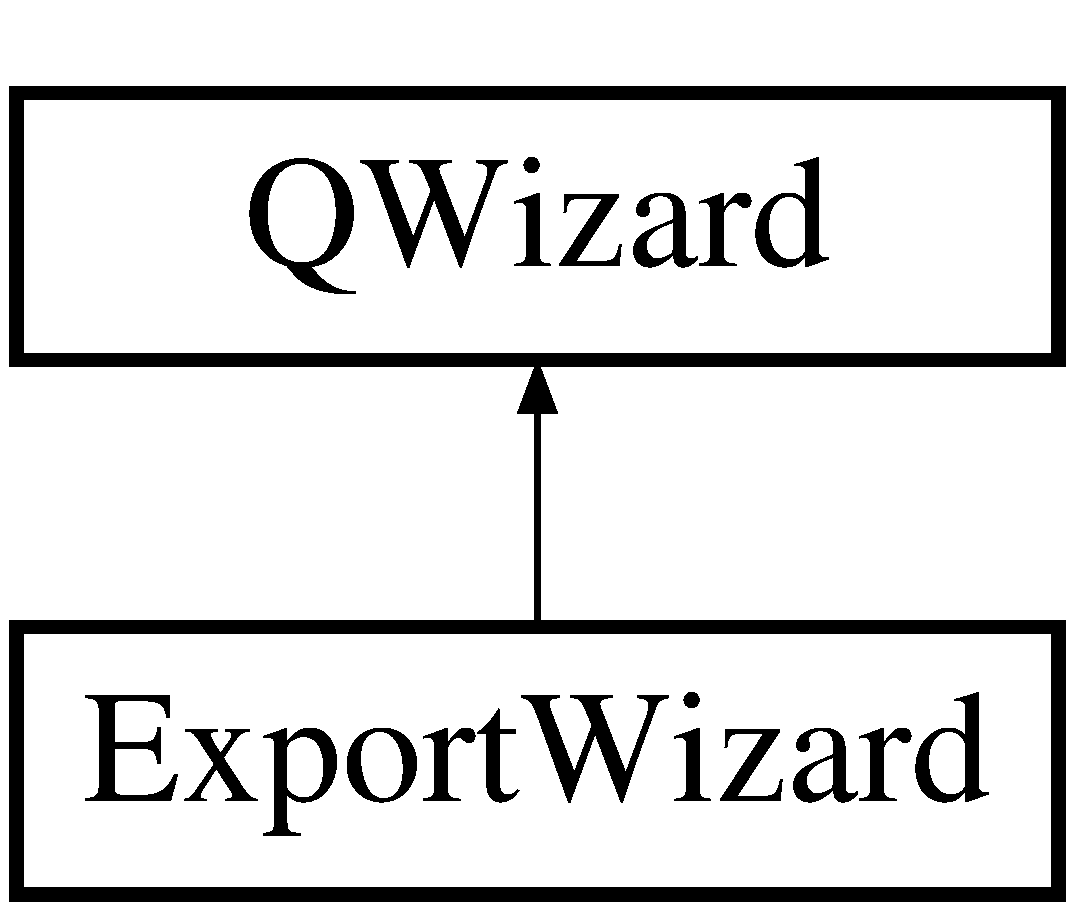
\includegraphics[height=2.000000cm]{class_export_wizard}
\end{center}
\end{figure}
\subsection*{Signals}
\begin{DoxyCompactItemize}
\item 
\hypertarget{class_export_wizard_aa27cd74a0821b70b2dd278ce519aa13e}{}void {\bfseries finished} ()\label{class_export_wizard_aa27cd74a0821b70b2dd278ce519aa13e}

\end{DoxyCompactItemize}
\subsection*{Public Member Functions}
\begin{DoxyCompactItemize}
\item 
\hypertarget{class_export_wizard_ae29f2a02ce3ae39857a17725f08dc6ba}{}{\bfseries Export\+Wizard} (Q\+Widget $\ast$parent=0)\label{class_export_wizard_ae29f2a02ce3ae39857a17725f08dc6ba}

\end{DoxyCompactItemize}
\subsection*{Public Attributes}
\begin{DoxyCompactItemize}
\item 
\hypertarget{class_export_wizard_af945c96c63098d827dd5eb684b568358}{}Q\+String {\bfseries format}\label{class_export_wizard_af945c96c63098d827dd5eb684b568358}

\item 
\hypertarget{class_export_wizard_a7d7df4c19102b7c04338cb5d7a169599}{}double {\bfseries vscale}\label{class_export_wizard_a7d7df4c19102b7c04338cb5d7a169599}

\item 
\hypertarget{class_export_wizard_a27bce3b2f0766e050c4da038d22453fd}{}int {\bfseries interval}\label{class_export_wizard_a27bce3b2f0766e050c4da038d22453fd}

\item 
\hypertarget{class_export_wizard_a02b2440bcb42d057cd8f327c9b985150}{}bool {\bfseries labels}\label{class_export_wizard_a02b2440bcb42d057cd8f327c9b985150}

\item 
\hypertarget{class_export_wizard_a74b5b1abb7991fab3663727dcad071b8}{}bool {\bfseries all\+Flows}\label{class_export_wizard_a74b5b1abb7991fab3663727dcad071b8}

\item 
\hypertarget{class_export_wizard_ac47c67db06c0d02cfaeab02c3629cd11}{}bool {\bfseries filter}\label{class_export_wizard_ac47c67db06c0d02cfaeab02c3629cd11}

\item 
\hypertarget{class_export_wizard_aa8d2e7cf93e56da19110cd6473fc7f5f}{}int {\bfseries color}\label{class_export_wizard_aa8d2e7cf93e56da19110cd6473fc7f5f}

\end{DoxyCompactItemize}
\subsection*{Protected Member Functions}
\begin{DoxyCompactItemize}
\item 
\hypertarget{class_export_wizard_a54cbfa3581936f77e15a65a0f328db15}{}bool \hyperlink{class_export_wizard_a54cbfa3581936f77e15a65a0f328db15}{validate\+Current\+Page} ()\label{class_export_wizard_a54cbfa3581936f77e15a65a0f328db15}

\begin{DoxyCompactList}\small\item\em called at page change \end{DoxyCompactList}\end{DoxyCompactItemize}
\subsection*{Private Attributes}
\begin{DoxyCompactItemize}
\item 
\hypertarget{class_export_wizard_aa041ae21b502041f8030f492dae16186}{}\hyperlink{class_ui_1_1_export_wizard}{Ui\+::\+Export\+Wizard} $\ast$ {\bfseries ui}\label{class_export_wizard_aa041ae21b502041f8030f492dae16186}

\end{DoxyCompactItemize}


The documentation for this class was generated from the following files\+:\begin{DoxyCompactItemize}
\item 
exportwizard.\+h\item 
exportwizard.\+cpp\item 
moc\+\_\+exportwizard.\+cpp\end{DoxyCompactItemize}

\hypertarget{class_ui_1_1_export_wizard}{}\section{Ui\+:\+:Export\+Wizard Class Reference}
\label{class_ui_1_1_export_wizard}\index{Ui\+::\+Export\+Wizard@{Ui\+::\+Export\+Wizard}}
Inheritance diagram for Ui\+:\+:Export\+Wizard\+:\begin{figure}[H]
\begin{center}
\leavevmode
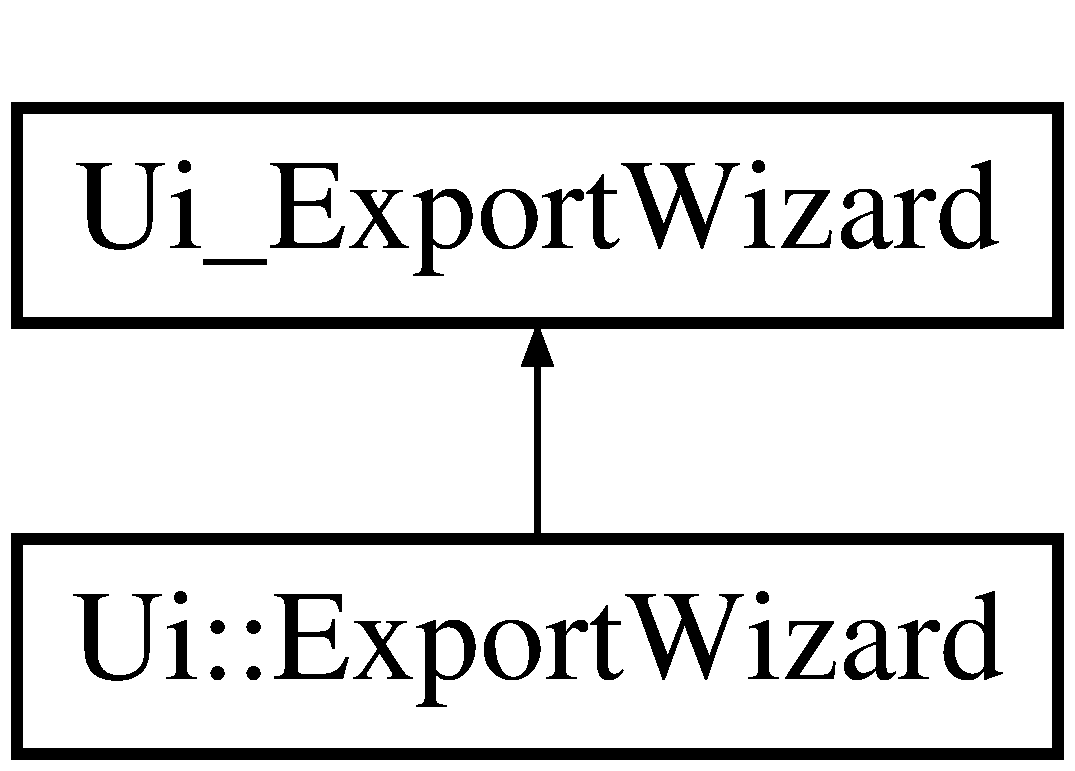
\includegraphics[height=2.000000cm]{class_ui_1_1_export_wizard}
\end{center}
\end{figure}
\subsection*{Additional Inherited Members}


The documentation for this class was generated from the following file\+:\begin{DoxyCompactItemize}
\item 
ui\+\_\+exportwizard.\+h\end{DoxyCompactItemize}

\hypertarget{struct_flow}{}\section{Flow Struct Reference}
\label{struct_flow}\index{Flow@{Flow}}


representation of a flow  




{\ttfamily \#include $<$mainwindow.\+h$>$}

\subsection*{Public Attributes}
\begin{DoxyCompactItemize}
\item 
\hypertarget{struct_flow_a0cc5ede8dd792ee075b3974ccc6c70e7}{}int \hyperlink{struct_flow_a0cc5ede8dd792ee075b3974ccc6c70e7}{flow\+Index}\label{struct_flow_a0cc5ede8dd792ee075b3974ccc6c70e7}

\begin{DoxyCompactList}\small\item\em The index of this flow in the \hyperlink{class_main_window_a843068e01d54730258357a4bc5f29bac}{Main\+Window\+::flows} list. \end{DoxyCompactList}\item 
\hypertarget{struct_flow_a3272e1f0ab6863ad902be6022fb9c537}{}int \hyperlink{struct_flow_a3272e1f0ab6863ad902be6022fb9c537}{unit1\+Index} = -\/1\label{struct_flow_a3272e1f0ab6863ad902be6022fb9c537}

\begin{DoxyCompactList}\small\item\em The index of the unit of the first \hyperlink{struct_task}{Task} in the \hyperlink{class_main_window_aad7505c53a0ad219080b3c1b1d1ef1e6}{Main\+Window\+::units} list. \end{DoxyCompactList}\item 
\hypertarget{struct_flow_a0e6209bf9cb7c20c6b3e8eff36c12527}{}int \hyperlink{struct_flow_a0e6209bf9cb7c20c6b3e8eff36c12527}{unit2\+Index} = -\/1\label{struct_flow_a0e6209bf9cb7c20c6b3e8eff36c12527}

\begin{DoxyCompactList}\small\item\em The index of the unit of the second \hyperlink{struct_task}{Task} in the \hyperlink{class_main_window_aad7505c53a0ad219080b3c1b1d1ef1e6}{Main\+Window\+::units} list. \end{DoxyCompactList}\item 
\hypertarget{struct_flow_a9f4a4871be5366c83e9d870781d396b6}{}int \hyperlink{struct_flow_a9f4a4871be5366c83e9d870781d396b6}{op1\+Index} = -\/1\label{struct_flow_a9f4a4871be5366c83e9d870781d396b6}

\begin{DoxyCompactList}\small\item\em The index of the first task in the \hyperlink{class_main_window_ab302362b256360d527a628bdbfcde171}{Main\+Window\+::tasks} list. \end{DoxyCompactList}\item 
\hypertarget{struct_flow_a42b73eff59dc5fc3e344ac5822280c57}{}int \hyperlink{struct_flow_a42b73eff59dc5fc3e344ac5822280c57}{op2\+Index} = -\/1\label{struct_flow_a42b73eff59dc5fc3e344ac5822280c57}

\begin{DoxyCompactList}\small\item\em The index of the second task in the \hyperlink{class_main_window_ab302362b256360d527a628bdbfcde171}{Main\+Window\+::tasks} list. \end{DoxyCompactList}\item 
\hypertarget{struct_flow_a381b8842d6e76fef6d17e78429562272}{}float \hyperlink{struct_flow_a381b8842d6e76fef6d17e78429562272}{amount}\label{struct_flow_a381b8842d6e76fef6d17e78429562272}

\begin{DoxyCompactList}\small\item\em The amount of this flow. \end{DoxyCompactList}\item 
\hypertarget{struct_flow_ae2bf28c63b4fe1e8d5681be424b59bec}{}float \hyperlink{struct_flow_ae2bf28c63b4fe1e8d5681be424b59bec}{production\+Rate}\label{struct_flow_ae2bf28c63b4fe1e8d5681be424b59bec}

\begin{DoxyCompactList}\small\item\em The production rate of this flow. \end{DoxyCompactList}\item 
\hypertarget{struct_flow_a4173165c2c3055d690d5e6584c66e5e6}{}float \hyperlink{struct_flow_a4173165c2c3055d690d5e6584c66e5e6}{consumption\+Rate}\label{struct_flow_a4173165c2c3055d690d5e6584c66e5e6}

\begin{DoxyCompactList}\small\item\em The consumption rate of this flow. \end{DoxyCompactList}\end{DoxyCompactItemize}


\subsection{Detailed Description}
representation of a flow 

The documentation for this struct was generated from the following file\+:\begin{DoxyCompactItemize}
\item 
mainwindow.\+h\end{DoxyCompactItemize}

\hypertarget{class_gantt_flow}{}\section{Gantt\+Flow Class Reference}
\label{class_gantt_flow}\index{Gantt\+Flow@{Gantt\+Flow}}
Inheritance diagram for Gantt\+Flow\+:\begin{figure}[H]
\begin{center}
\leavevmode
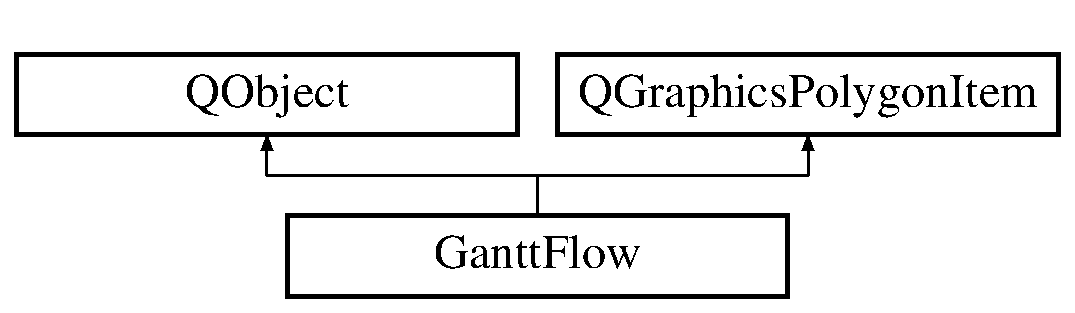
\includegraphics[height=2.000000cm]{class_gantt_flow}
\end{center}
\end{figure}
\subsection*{Signals}
\begin{DoxyCompactItemize}
\item 
\hypertarget{class_gantt_flow_ac70e8aa9713b3f9491c005e432b27cf3}{}void {\bfseries i\+Was\+Clicked} (int index)\label{class_gantt_flow_ac70e8aa9713b3f9491c005e432b27cf3}

\end{DoxyCompactItemize}
\subsection*{Public Member Functions}
\begin{DoxyCompactItemize}
\item 
\hypertarget{class_gantt_flow_a049bba5800cffb959fc25b956611e0dd}{}{\bfseries Gantt\+Flow} (int flow\+Index, Q\+Polygon\+F points, Q\+Graphics\+Item $\ast$parent=0)\label{class_gantt_flow_a049bba5800cffb959fc25b956611e0dd}

\item 
\hypertarget{class_gantt_flow_aa15236657e635084fdd7d17209949fcd}{}void {\bfseries is\+Selected} ()\label{class_gantt_flow_aa15236657e635084fdd7d17209949fcd}

\item 
\hypertarget{class_gantt_flow_a5b4f74ffc39282abc9d109f104031201}{}void {\bfseries is\+Not\+Selected} ()\label{class_gantt_flow_a5b4f74ffc39282abc9d109f104031201}

\end{DoxyCompactItemize}
\subsection*{Protected Member Functions}
\begin{DoxyCompactItemize}
\item 
\hypertarget{class_gantt_flow_a71c4e6b658663c3bf916bf9eadc444e3}{}void {\bfseries mouse\+Press\+Event} (Q\+Graphics\+Scene\+Mouse\+Event $\ast$event)\label{class_gantt_flow_a71c4e6b658663c3bf916bf9eadc444e3}

\end{DoxyCompactItemize}
\subsection*{Private Attributes}
\begin{DoxyCompactItemize}
\item 
\hypertarget{class_gantt_flow_adad338ed721f9d3881da17042c2cd66f}{}int {\bfseries flow\+Index}\label{class_gantt_flow_adad338ed721f9d3881da17042c2cd66f}

\end{DoxyCompactItemize}


The documentation for this class was generated from the following files\+:\begin{DoxyCompactItemize}
\item 
ganttflow.\+h\item 
ganttflow.\+cpp\item 
moc\+\_\+ganttflow.\+cpp\end{DoxyCompactItemize}

\hypertarget{class_gantt_graphics_view}{}\section{Gantt\+Graphics\+View Class Reference}
\label{class_gantt_graphics_view}\index{Gantt\+Graphics\+View@{Gantt\+Graphics\+View}}
Inheritance diagram for Gantt\+Graphics\+View\+:\begin{figure}[H]
\begin{center}
\leavevmode
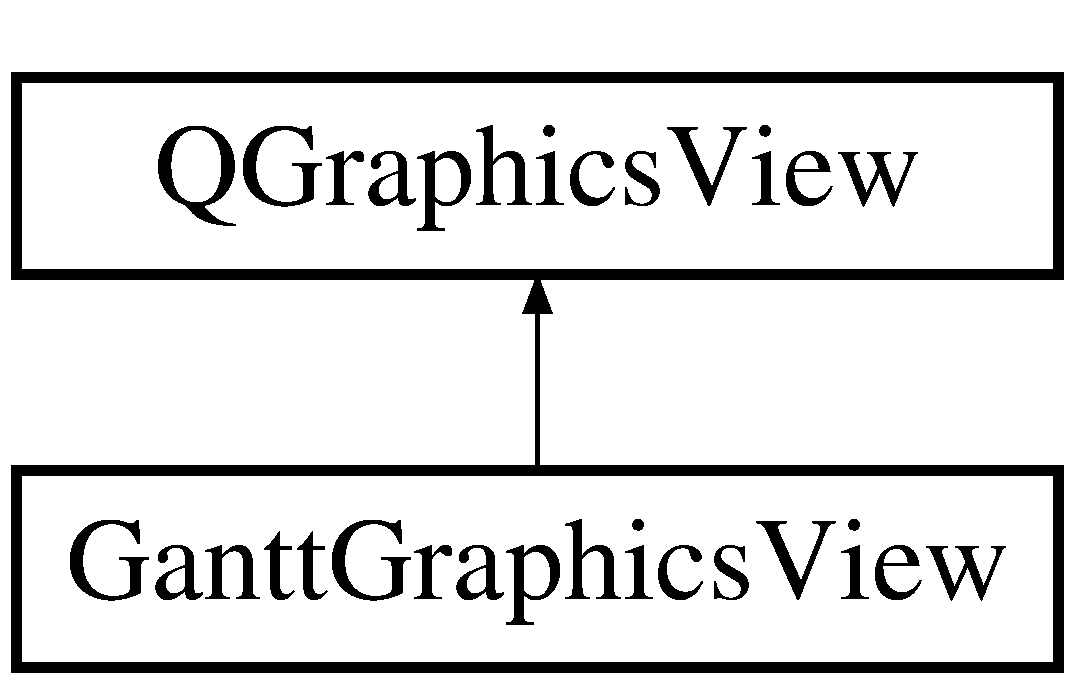
\includegraphics[height=2.000000cm]{class_gantt_graphics_view}
\end{center}
\end{figure}
\subsection*{Public Attributes}
\begin{DoxyCompactItemize}
\item 
\hypertarget{class_gantt_graphics_view_a9f75c7c70ff0f5ed86851b2568e0761f}{}Q\+Graphics\+Scene $\ast$ {\bfseries scene}\label{class_gantt_graphics_view_a9f75c7c70ff0f5ed86851b2568e0761f}

\item 
\hypertarget{class_gantt_graphics_view_a4bdcbe149a72ebf613c3b20194af1177}{}Q\+List$<$ \hyperlink{class_gantt_rect}{Gantt\+Rect} $\ast$ $>$ $\ast$ {\bfseries tasks}\label{class_gantt_graphics_view_a4bdcbe149a72ebf613c3b20194af1177}

\item 
\hypertarget{class_gantt_graphics_view_a1b2317941c3cc0d46f487150f9a23345}{}Q\+List$<$ \hyperlink{class_gantt_flow}{Gantt\+Flow} $\ast$ $>$ $\ast$ {\bfseries flows}\label{class_gantt_graphics_view_a1b2317941c3cc0d46f487150f9a23345}

\item 
\hypertarget{class_gantt_graphics_view_a024da97a8f64fe1a93ac8f66ebd0c509}{}Q\+List$<$ Q\+Graphics\+Line\+Item $\ast$ $>$ $\ast$ {\bfseries lines}\label{class_gantt_graphics_view_a024da97a8f64fe1a93ac8f66ebd0c509}

\item 
\hypertarget{class_gantt_graphics_view_a0c9e18df143ee370ef16ad191ec89243}{}Q\+List$<$ Q\+Graphics\+Text\+Item $\ast$ $>$ $\ast$ {\bfseries unit\+Labels}\label{class_gantt_graphics_view_a0c9e18df143ee370ef16ad191ec89243}

\end{DoxyCompactItemize}
\subsection*{Protected Member Functions}
\begin{DoxyCompactItemize}
\item 
\hypertarget{class_gantt_graphics_view_a839f61e2646f059eb29c7b3a1e6ca15e}{}void {\bfseries resize\+Event} (Q\+Resize\+Event $\ast$event)\label{class_gantt_graphics_view_a839f61e2646f059eb29c7b3a1e6ca15e}

\item 
\hypertarget{class_gantt_graphics_view_a31beb77537b5418c5f6dea00908b4f3b}{}void {\bfseries key\+Press\+Event} (Q\+Key\+Event $\ast$e)\label{class_gantt_graphics_view_a31beb77537b5418c5f6dea00908b4f3b}

\item 
\hypertarget{class_gantt_graphics_view_a4f89078a1ee9352fe08118664a9bfca1}{}void {\bfseries key\+Release\+Event} (Q\+Key\+Event $\ast$e)\label{class_gantt_graphics_view_a4f89078a1ee9352fe08118664a9bfca1}

\end{DoxyCompactItemize}


The documentation for this class was generated from the following files\+:\begin{DoxyCompactItemize}
\item 
ganttgraphicsview.\+h\item 
ganttgraphicsview.\+cpp\end{DoxyCompactItemize}

\hypertarget{class_gantt_line}{}\section{Gantt\+Line Class Reference}
\label{class_gantt_line}\index{Gantt\+Line@{Gantt\+Line}}
Inheritance diagram for Gantt\+Line\+:\begin{figure}[H]
\begin{center}
\leavevmode
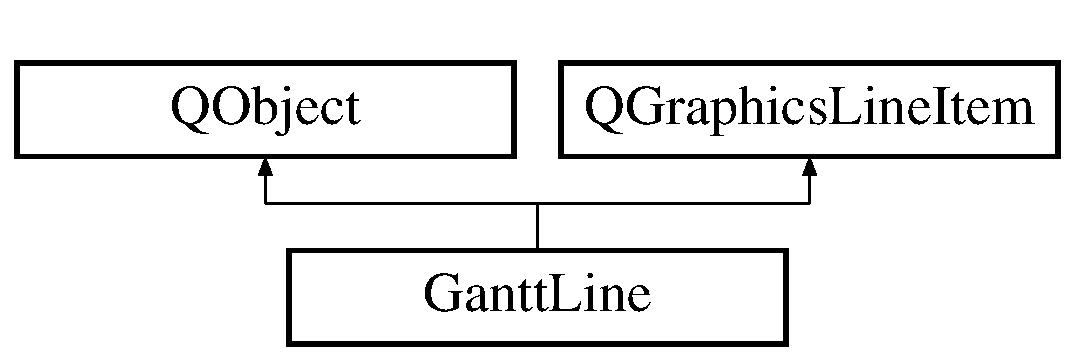
\includegraphics[height=2.000000cm]{class_gantt_line}
\end{center}
\end{figure}
\subsection*{Signals}
\begin{DoxyCompactItemize}
\item 
\hypertarget{class_gantt_line_a21a3f4419468070e64b1abe0ba882a93}{}void {\bfseries i\+Was\+Clicked} (int index)\label{class_gantt_line_a21a3f4419468070e64b1abe0ba882a93}

\end{DoxyCompactItemize}
\subsection*{Public Member Functions}
\begin{DoxyCompactItemize}
\item 
\hypertarget{class_gantt_line_a9551c71e45c4d5d297d18e13701a624a}{}{\bfseries Gantt\+Line} (int flow\+Index, qreal x1, qreal y1, qreal x2, qreal y2, Q\+Graphics\+Item $\ast$parent=Q\+\_\+\+N\+U\+L\+L\+P\+T\+R)\label{class_gantt_line_a9551c71e45c4d5d297d18e13701a624a}

\end{DoxyCompactItemize}
\subsection*{Protected Member Functions}
\begin{DoxyCompactItemize}
\item 
\hypertarget{class_gantt_line_a9c8c663fbf70ef48ca8135be86f6e48b}{}void {\bfseries mouse\+Press\+Event} (Q\+Graphics\+Scene\+Mouse\+Event $\ast$event)\label{class_gantt_line_a9c8c663fbf70ef48ca8135be86f6e48b}

\end{DoxyCompactItemize}
\subsection*{Private Attributes}
\begin{DoxyCompactItemize}
\item 
\hypertarget{class_gantt_line_afdc3b8ef93711d3a20dce12d50b4460f}{}int {\bfseries flow\+Index}\label{class_gantt_line_afdc3b8ef93711d3a20dce12d50b4460f}

\end{DoxyCompactItemize}


The documentation for this class was generated from the following files\+:\begin{DoxyCompactItemize}
\item 
ganttline.\+h\item 
ganttline.\+cpp\item 
moc\+\_\+ganttline.\+cpp\end{DoxyCompactItemize}

\hypertarget{class_gantt_rect}{}\section{Gantt\+Rect Class Reference}
\label{class_gantt_rect}\index{Gantt\+Rect@{Gantt\+Rect}}
Inheritance diagram for Gantt\+Rect\+:\begin{figure}[H]
\begin{center}
\leavevmode
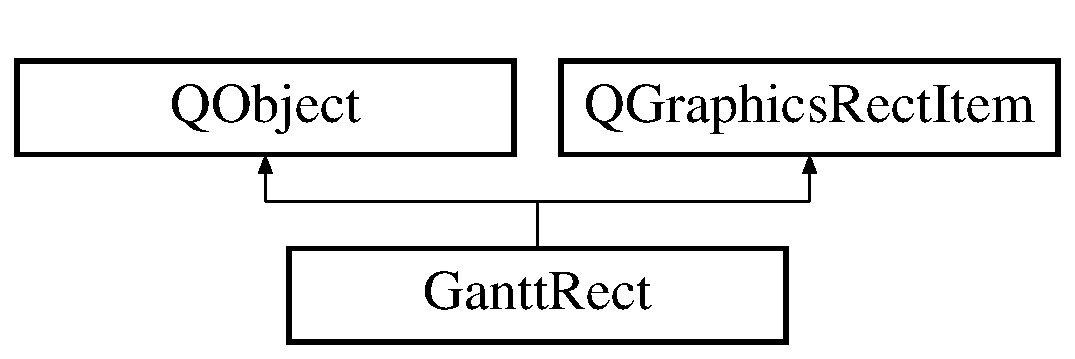
\includegraphics[height=2.000000cm]{class_gantt_rect}
\end{center}
\end{figure}
\subsection*{Signals}
\begin{DoxyCompactItemize}
\item 
\hypertarget{class_gantt_rect_a145e1920586490aa4d42d17c5f6c550c}{}void {\bfseries i\+Was\+Clicked} (int index)\label{class_gantt_rect_a145e1920586490aa4d42d17c5f6c550c}

\item 
\hypertarget{class_gantt_rect_af0d26710b0714d23877baf60448612ee}{}void {\bfseries hover\+Start} (int index)\label{class_gantt_rect_af0d26710b0714d23877baf60448612ee}

\item 
\hypertarget{class_gantt_rect_a7b68e31966743b4627919f14bcc3d33d}{}void {\bfseries hover\+Leave} (int index)\label{class_gantt_rect_a7b68e31966743b4627919f14bcc3d33d}

\end{DoxyCompactItemize}
\subsection*{Public Member Functions}
\begin{DoxyCompactItemize}
\item 
\hypertarget{class_gantt_rect_a1796a2b89044eda5d417236b9605e8db}{}{\bfseries Gantt\+Rect} (int task\+Index, int unit\+Index, float largest\+Amount, float start, float end, float amount, Q\+Color color, Q\+Graphics\+Item $\ast$parent=Q\+\_\+\+N\+U\+L\+L\+P\+T\+R)\label{class_gantt_rect_a1796a2b89044eda5d417236b9605e8db}

\item 
\hypertarget{class_gantt_rect_ab56a963d676eaa923430bb940390e017}{}void {\bfseries show\+Amount} (bool yes)\label{class_gantt_rect_ab56a963d676eaa923430bb940390e017}

\item 
\hypertarget{class_gantt_rect_aebb14eb8a807a0e5d560c311c81961c3}{}void {\bfseries is\+Selected} ()\label{class_gantt_rect_aebb14eb8a807a0e5d560c311c81961c3}

\item 
\hypertarget{class_gantt_rect_a1681372c908aaab78c22beaf4146a432}{}void {\bfseries is\+Not\+Selected} ()\label{class_gantt_rect_a1681372c908aaab78c22beaf4146a432}

\item 
\hypertarget{class_gantt_rect_a3d470a764ab8a79c08502d8c92859f88}{}void {\bfseries is\+Marked\+In\+Flow} ()\label{class_gantt_rect_a3d470a764ab8a79c08502d8c92859f88}

\item 
\hypertarget{class_gantt_rect_a769aacba6fa021fe98b8b53f29873851}{}void {\bfseries is\+Not\+Marked\+In\+Flow} ()\label{class_gantt_rect_a769aacba6fa021fe98b8b53f29873851}

\item 
\hypertarget{class_gantt_rect_ac4190e95053e095f83874ba41b0e18a2}{}void {\bfseries blink} ()\label{class_gantt_rect_ac4190e95053e095f83874ba41b0e18a2}

\end{DoxyCompactItemize}
\subsection*{Public Attributes}
\begin{DoxyCompactItemize}
\item 
\hypertarget{class_gantt_rect_a6642ac413af5ade187fac723016f8292}{}int {\bfseries task\+Index}\label{class_gantt_rect_a6642ac413af5ade187fac723016f8292}

\item 
\hypertarget{class_gantt_rect_aad3beda6dc33e7144632705476e2745a}{}int {\bfseries unit\+Index}\label{class_gantt_rect_aad3beda6dc33e7144632705476e2745a}

\end{DoxyCompactItemize}
\subsection*{Protected Member Functions}
\begin{DoxyCompactItemize}
\item 
\hypertarget{class_gantt_rect_a86e51a147edf6df229f1aad0a5089481}{}void {\bfseries mouse\+Press\+Event} (Q\+Graphics\+Scene\+Mouse\+Event $\ast$event)\label{class_gantt_rect_a86e51a147edf6df229f1aad0a5089481}

\item 
\hypertarget{class_gantt_rect_ad98eae638288375964942f34c4d315de}{}void {\bfseries hover\+Enter\+Event} (Q\+Graphics\+Scene\+Hover\+Event $\ast$event)\label{class_gantt_rect_ad98eae638288375964942f34c4d315de}

\item 
\hypertarget{class_gantt_rect_a3b2e69fe42463cedddb5e3cd8c2a88b1}{}void {\bfseries hover\+Leave\+Event} (Q\+Graphics\+Scene\+Hover\+Event $\ast$event)\label{class_gantt_rect_a3b2e69fe42463cedddb5e3cd8c2a88b1}

\end{DoxyCompactItemize}
\subsection*{Private Attributes}
\begin{DoxyCompactItemize}
\item 
\hypertarget{class_gantt_rect_a87c303488aa50b2b26dacc4641a50ccb}{}float {\bfseries largest\+Amount}\label{class_gantt_rect_a87c303488aa50b2b26dacc4641a50ccb}

\item 
\hypertarget{class_gantt_rect_a0146f1175f8a38f825f7bc0dd9ead993}{}float {\bfseries start}\label{class_gantt_rect_a0146f1175f8a38f825f7bc0dd9ead993}

\item 
\hypertarget{class_gantt_rect_aa730838f983a964aecd07f1888703841}{}float {\bfseries end}\label{class_gantt_rect_aa730838f983a964aecd07f1888703841}

\item 
\hypertarget{class_gantt_rect_a49e581012b987f5038403b25427dabe7}{}float {\bfseries amount}\label{class_gantt_rect_a49e581012b987f5038403b25427dabe7}

\item 
\hypertarget{class_gantt_rect_a6ed153f381b086ad680e83da17662886}{}Q\+Pen {\bfseries pen}\label{class_gantt_rect_a6ed153f381b086ad680e83da17662886}

\end{DoxyCompactItemize}


The documentation for this class was generated from the following files\+:\begin{DoxyCompactItemize}
\item 
ganttrect.\+h\item 
ganttrect.\+cpp\item 
moc\+\_\+ganttrect.\+cpp\end{DoxyCompactItemize}

\hypertarget{class_main_window}{}\section{Main\+Window Class Reference}
\label{class_main_window}\index{Main\+Window@{Main\+Window}}


Class for the Main window.  




{\ttfamily \#include $<$mainwindow.\+h$>$}

Inheritance diagram for Main\+Window\+:\begin{figure}[H]
\begin{center}
\leavevmode
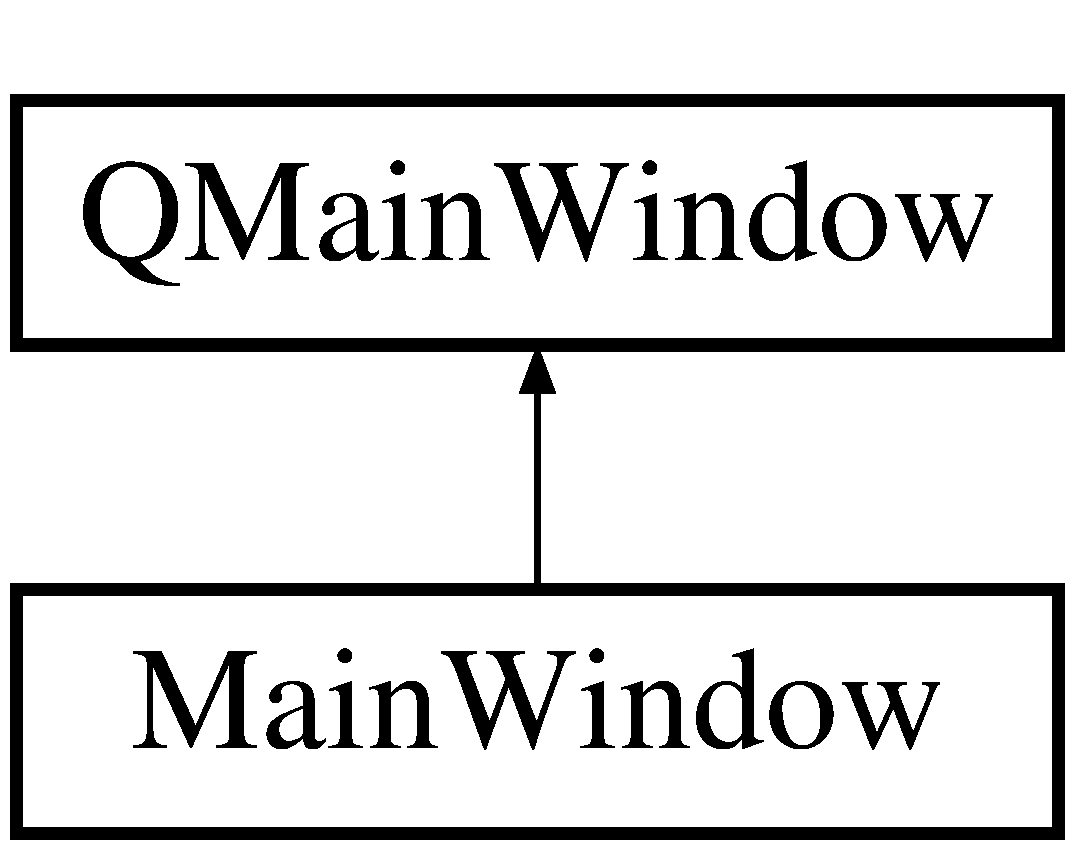
\includegraphics[height=2.000000cm]{class_main_window}
\end{center}
\end{figure}
\subsection*{Public Member Functions}
\begin{DoxyCompactItemize}
\item 
\hypertarget{class_main_window_a8b244be8b7b7db1b08de2a2acb9409db}{}{\bfseries Main\+Window} (Q\+Widget $\ast$parent=0)\label{class_main_window_a8b244be8b7b7db1b08de2a2acb9409db}

\item 
\hypertarget{class_main_window_a75d7910a13ccc8ee60126bf7be448341}{}bool {\bfseries event\+Filter} (Q\+Object $\ast$watched, Q\+Event $\ast$event)\label{class_main_window_a75d7910a13ccc8ee60126bf7be448341}

\end{DoxyCompactItemize}
\subsection*{Protected Member Functions}
\begin{DoxyCompactItemize}
\item 
\hypertarget{class_main_window_ae12f8f63791595567b6250f8bb002bda}{}void {\bfseries resize\+Event} (Q\+Resize\+Event $\ast$event)\label{class_main_window_ae12f8f63791595567b6250f8bb002bda}

\item 
\hypertarget{class_main_window_adf88315e557e377353059bd313b1bfa6}{}void {\bfseries key\+Press\+Event} (Q\+Key\+Event $\ast$e)\label{class_main_window_adf88315e557e377353059bd313b1bfa6}

\item 
\hypertarget{class_main_window_a04b0c8ff3be04d1b1bf54e78c5ee7039}{}void {\bfseries key\+Release\+Event} (Q\+Key\+Event $\ast$e)\label{class_main_window_a04b0c8ff3be04d1b1bf54e78c5ee7039}

\item 
\hypertarget{class_main_window_ad2a20182d1ed20479debef57417cdb05}{}void {\bfseries wheel\+Event} (Q\+Wheel\+Event $\ast$e)\label{class_main_window_ad2a20182d1ed20479debef57417cdb05}

\end{DoxyCompactItemize}
\subsection*{Private Slots}
\begin{DoxyCompactItemize}
\item 
\hypertarget{class_main_window_a4878ed6cf33c2814e8a7c89e894585bc}{}void \hyperlink{class_main_window_a4878ed6cf33c2814e8a7c89e894585bc}{vertical\+Zoom\+Slider\+Changed} (int x)\label{class_main_window_a4878ed6cf33c2814e8a7c89e894585bc}

\begin{DoxyCompactList}\small\item\em called when the vertical zoom slider changed \end{DoxyCompactList}\item 
\hypertarget{class_main_window_a181da03c02e690223c8f93fe558bb4df}{}void \hyperlink{class_main_window_a181da03c02e690223c8f93fe558bb4df}{horizontal\+Zoom\+Slider\+Changed} (int x)\label{class_main_window_a181da03c02e690223c8f93fe558bb4df}

\begin{DoxyCompactList}\small\item\em called when the horizontal zoom slider changed \end{DoxyCompactList}\item 
\hypertarget{class_main_window_a1bce12a42d710ac9e5afa4d1a0a9aa4b}{}void \hyperlink{class_main_window_a1bce12a42d710ac9e5afa4d1a0a9aa4b}{v\+\_\+zoomin} ()\label{class_main_window_a1bce12a42d710ac9e5afa4d1a0a9aa4b}

\begin{DoxyCompactList}\small\item\em zoom in vertically by 2x \end{DoxyCompactList}\item 
\hypertarget{class_main_window_a9d72b029178eab9350387aa85d608add}{}void \hyperlink{class_main_window_a9d72b029178eab9350387aa85d608add}{v\+\_\+zoomout} ()\label{class_main_window_a9d72b029178eab9350387aa85d608add}

\begin{DoxyCompactList}\small\item\em zoom out vertically by 2x \end{DoxyCompactList}\item 
\hypertarget{class_main_window_ad6d9b74f56b82f77078c2c656abc418b}{}void \hyperlink{class_main_window_ad6d9b74f56b82f77078c2c656abc418b}{h\+\_\+zoomin} ()\label{class_main_window_ad6d9b74f56b82f77078c2c656abc418b}

\begin{DoxyCompactList}\small\item\em zoom in horizontally by 2x \end{DoxyCompactList}\item 
\hypertarget{class_main_window_a777aff65da0144d1ed34646518ea955a}{}void \hyperlink{class_main_window_a777aff65da0144d1ed34646518ea955a}{h\+\_\+zoomout} ()\label{class_main_window_a777aff65da0144d1ed34646518ea955a}

\begin{DoxyCompactList}\small\item\em zoom out horizontally by 2x \end{DoxyCompactList}\item 
\hypertarget{class_main_window_a0c980716d7ece94ad4e01921ce557e98}{}void \hyperlink{class_main_window_a0c980716d7ece94ad4e01921ce557e98}{task\+Clicked} (int index)\label{class_main_window_a0c980716d7ece94ad4e01921ce557e98}

\begin{DoxyCompactList}\small\item\em called when a task ( its graphical representation as a \hyperlink{class_gantt_rect}{Gantt\+Rect} ) has been clicked \end{DoxyCompactList}\item 
\hypertarget{class_main_window_a2d3ef18f661856ebd7f1ee149e95c900}{}void \hyperlink{class_main_window_a2d3ef18f661856ebd7f1ee149e95c900}{task\+Hover\+Enter} (int index)\label{class_main_window_a2d3ef18f661856ebd7f1ee149e95c900}

\begin{DoxyCompactList}\small\item\em called when a task ( its graphical representation as a \hyperlink{class_gantt_rect}{Gantt\+Rect} ) has started being hovered on \end{DoxyCompactList}\item 
\hypertarget{class_main_window_a3a3957874de63e80e41661860e2b12c3}{}void \hyperlink{class_main_window_a3a3957874de63e80e41661860e2b12c3}{task\+Hover\+Leave} (int index)\label{class_main_window_a3a3957874de63e80e41661860e2b12c3}

\begin{DoxyCompactList}\small\item\em called when a task ( its graphical representation as a \hyperlink{class_gantt_rect}{Gantt\+Rect} ) has stopped being hovered on \end{DoxyCompactList}\item 
\hypertarget{class_main_window_aec3a0dff06eb089dbf3d8c4175d8e004}{}void \hyperlink{class_main_window_aec3a0dff06eb089dbf3d8c4175d8e004}{flow\+Clicked} (int index)\label{class_main_window_aec3a0dff06eb089dbf3d8c4175d8e004}

\begin{DoxyCompactList}\small\item\em called when a flow ( its graphical representation as a \hyperlink{class_gantt_flow}{Gantt\+Flow} ) has been clicked \end{DoxyCompactList}\item 
\hypertarget{class_main_window_abacc539de6f25ca81a6b0543be799155}{}void \hyperlink{class_main_window_abacc539de6f25ca81a6b0543be799155}{task\+Table\+Clicked} (int index, int \+\_\+)\label{class_main_window_abacc539de6f25ca81a6b0543be799155}

\begin{DoxyCompactList}\small\item\em called when a task has been selected in the table \end{DoxyCompactList}\item 
\hypertarget{class_main_window_a580a35d29abc0a0c82edf183e7f87b74}{}void \hyperlink{class_main_window_a580a35d29abc0a0c82edf183e7f87b74}{open\+C\+S\+V} ()\label{class_main_window_a580a35d29abc0a0c82edf183e7f87b74}

\begin{DoxyCompactList}\small\item\em called by open\+C\+S\+V\+Act, opens a File selection window and parses the selected C\+S\+V file. \end{DoxyCompactList}\item 
\hypertarget{class_main_window_a23e9c749c8f0e5119317ea6484b9476f}{}void \hyperlink{class_main_window_a23e9c749c8f0e5119317ea6484b9476f}{open\+G\+D\+X} ()\label{class_main_window_a23e9c749c8f0e5119317ea6484b9476f}

\begin{DoxyCompactList}\small\item\em called by open\+G\+D\+X\+Act, opens a \hyperlink{class_wizard}{Wizard} for reading G\+D\+X files. \end{DoxyCompactList}\item 
\hypertarget{class_main_window_a631ac3f30fb6a0b0dc441739f0abe624}{}void \hyperlink{class_main_window_a631ac3f30fb6a0b0dc441739f0abe624}{visualizeamounts} ()\label{class_main_window_a631ac3f30fb6a0b0dc441739f0abe624}

\begin{DoxyCompactList}\small\item\em called by visualize\+Amounts\+Act \end{DoxyCompactList}\item 
\hypertarget{class_main_window_a36b4cda2f78374242c8fed56634dff90}{}void \hyperlink{class_main_window_a36b4cda2f78374242c8fed56634dff90}{show\+All\+Flows\+Toggled} ()\label{class_main_window_a36b4cda2f78374242c8fed56634dff90}

\begin{DoxyCompactList}\small\item\em called by show\+All\+Flows\+Act \end{DoxyCompactList}\item 
\hypertarget{class_main_window_aa01206c494495bf0dc61d5dd1adf3ef7}{}void {\bfseries scrolln} ()\label{class_main_window_aa01206c494495bf0dc61d5dd1adf3ef7}

\item 
\hypertarget{class_main_window_aedee761ccc4e5677bd1d3f37047b8809}{}void {\bfseries scrolle} ()\label{class_main_window_aedee761ccc4e5677bd1d3f37047b8809}

\item 
\hypertarget{class_main_window_a09f8db735147f5631d706aa7e3cff52c}{}void {\bfseries scrolls} ()\label{class_main_window_a09f8db735147f5631d706aa7e3cff52c}

\item 
\hypertarget{class_main_window_aaaec2945183e4bee42128478b2b66602}{}void {\bfseries scrollw} ()\label{class_main_window_aaaec2945183e4bee42128478b2b66602}

\item 
\hypertarget{class_main_window_af781f827f0e0df1357044a1861568600}{}void {\bfseries center} ()\label{class_main_window_af781f827f0e0df1357044a1861568600}

\item 
\hypertarget{class_main_window_aa74202e1272a25d59ff3799a48182b80}{}void {\bfseries check} ()\label{class_main_window_aa74202e1272a25d59ff3799a48182b80}

\item 
\hypertarget{class_main_window_a267eecc8fffb48d32f449d83d6604dd7}{}void \hyperlink{class_main_window_a267eecc8fffb48d32f449d83d6604dd7}{save\+Logs} ()\label{class_main_window_a267eecc8fffb48d32f449d83d6604dd7}

\begin{DoxyCompactList}\small\item\em Save log ouput to file. \end{DoxyCompactList}\item 
\hypertarget{class_main_window_a0cffe7069f97c1795a8ba7f00002f43e}{}void {\bfseries color\+By\+Amount} ()\label{class_main_window_a0cffe7069f97c1795a8ba7f00002f43e}

\item 
\hypertarget{class_main_window_a1f40b9a1fd5872645aaf1e9e3fe82a45}{}void {\bfseries color\+By\+Unit} ()\label{class_main_window_a1f40b9a1fd5872645aaf1e9e3fe82a45}

\item 
\hypertarget{class_main_window_a4e71a4c397c36e151a917039c7db06d7}{}void {\bfseries color\+By\+Color} ()\label{class_main_window_a4e71a4c397c36e151a917039c7db06d7}

\item 
\hypertarget{class_main_window_a5e7373649a8fdcd8fc010c321569864a}{}void {\bfseries color\+By\+Task} ()\label{class_main_window_a5e7373649a8fdcd8fc010c321569864a}

\item 
\hypertarget{class_main_window_a494c17acd55c3f4c1ccf1710371bb322}{}void {\bfseries export\+To\+Image} ()\label{class_main_window_a494c17acd55c3f4c1ccf1710371bb322}

\item 
\hypertarget{class_main_window_a19794f4b42e03bee539fd9783825a3b6}{}void {\bfseries rule\+Changed\+Amount} (int index)\label{class_main_window_a19794f4b42e03bee539fd9783825a3b6}

\item 
\hypertarget{class_main_window_a462222b03801d153d7e1eaf037741dd7}{}void {\bfseries rule\+Changed\+Duration} (int index)\label{class_main_window_a462222b03801d153d7e1eaf037741dd7}

\item 
\hypertarget{class_main_window_a243f90594158b9d2b14bec0fbf192b13}{}void {\bfseries rule\+Changed\+Start} (int index)\label{class_main_window_a243f90594158b9d2b14bec0fbf192b13}

\item 
\hypertarget{class_main_window_a5a4b524f33975847930b136d0e497958}{}void {\bfseries rule\+Changed\+End} (int index)\label{class_main_window_a5a4b524f33975847930b136d0e497958}

\item 
\hypertarget{class_main_window_acecada8d60710fb12ef90f8752f7f074}{}void {\bfseries apply\+Filter} ()\label{class_main_window_acecada8d60710fb12ef90f8752f7f074}

\item 
\hypertarget{class_main_window_ade9c4f4c00ac1956276e10e65123b848}{}void {\bfseries clear\+Filter} ()\label{class_main_window_ade9c4f4c00ac1956276e10e65123b848}

\item 
\hypertarget{class_main_window_a0b3d1510d0e0ed665daa74d6823e00d6}{}void \hyperlink{class_main_window_a0b3d1510d0e0ed665daa74d6823e00d6}{create\+Representation} ()\label{class_main_window_a0b3d1510d0e0ed665daa74d6823e00d6}

\begin{DoxyCompactList}\small\item\em Creates the graphical representation of the gantt chart. \end{DoxyCompactList}\item 
\hypertarget{class_main_window_a645f1cd085c2636dc4eccb320455a6f4}{}void \hyperlink{class_main_window_a645f1cd085c2636dc4eccb320455a6f4}{add\+Flow} (Q\+String unit1name, Q\+String op1name, Q\+String unit2name, Q\+String op2name, float pr, float cr, float amount)\label{class_main_window_a645f1cd085c2636dc4eccb320455a6f4}

\begin{DoxyCompactList}\small\item\em Adds a \hyperlink{struct_flow}{Flow} to the flows list. \end{DoxyCompactList}\item 
\hypertarget{class_main_window_a2920d5c6c64925cb5f87c7fdac3f54b0}{}void \hyperlink{class_main_window_a2920d5c6c64925cb5f87c7fdac3f54b0}{add\+Task} (Q\+String unit\+Name, Q\+String task\+Name, float start, float end, float amount, Q\+String color=\char`\"{}random\char`\"{})\label{class_main_window_a2920d5c6c64925cb5f87c7fdac3f54b0}

\begin{DoxyCompactList}\small\item\em Adds a \hyperlink{struct_task}{Task} to the tasks list. color is a color name in hex format, if none is given a random color will be generated. \end{DoxyCompactList}\item 
\hypertarget{class_main_window_a02076de46e6810174817ebfc6ddd2be5}{}void \hyperlink{class_main_window_a02076de46e6810174817ebfc6ddd2be5}{reset} ()\label{class_main_window_a02076de46e6810174817ebfc6ddd2be5}

\begin{DoxyCompactList}\small\item\em reset the window (important for loading new files) \end{DoxyCompactList}\end{DoxyCompactItemize}
\subsection*{Private Member Functions}
\begin{DoxyCompactItemize}
\item 
\hypertarget{class_main_window_a6a403614bd858e16e35af405c562fc9b}{}void {\bfseries reset\+Zoom} ()\label{class_main_window_a6a403614bd858e16e35af405c562fc9b}

\item 
\hypertarget{class_main_window_aa9bca4a0b90acf75f82a7f1acc411acb}{}void \hyperlink{class_main_window_aa9bca4a0b90acf75f82a7f1acc411acb}{show\+Flows} (int task\+Index)\label{class_main_window_aa9bca4a0b90acf75f82a7f1acc411acb}

\begin{DoxyCompactList}\small\item\em Recursively make all flows connected to this task visible. \end{DoxyCompactList}\item 
\hypertarget{class_main_window_a8c5ff24ebba239b7dbf435b3dd50e1f3}{}void {\bfseries recursively\+Activate\+Flows\+To\+The\+Right} (int task\+Index)\label{class_main_window_a8c5ff24ebba239b7dbf435b3dd50e1f3}

\item 
\hypertarget{class_main_window_af938550e53f022625dd21ff1536bb36b}{}void {\bfseries recursively\+Activate\+Flows\+To\+The\+Left} (int task\+Index)\label{class_main_window_af938550e53f022625dd21ff1536bb36b}

\item 
\hypertarget{class_main_window_a63772da55576703fd979ced117a9fa89}{}void \hyperlink{class_main_window_a63772da55576703fd979ced117a9fa89}{show\+Amount} (bool yes)\label{class_main_window_a63772da55576703fd979ced117a9fa89}

\begin{DoxyCompactList}\small\item\em Set wether to visualize amounts by height. \end{DoxyCompactList}\item 
\hypertarget{class_main_window_a28e45b950a89e35ffb5b1d1e345e7aa6}{}void \hyperlink{class_main_window_a28e45b950a89e35ffb5b1d1e345e7aa6}{select\+Task\+On\+Table} (int index)\label{class_main_window_a28e45b950a89e35ffb5b1d1e345e7aa6}

\begin{DoxyCompactList}\small\item\em select a \hyperlink{struct_task}{Task} in the Table by index \end{DoxyCompactList}\item 
\hypertarget{class_main_window_a03799692902ab88a551b4dca1fa042db}{}void \hyperlink{class_main_window_a03799692902ab88a551b4dca1fa042db}{create\+Menu} ()\label{class_main_window_a03799692902ab88a551b4dca1fa042db}

\begin{DoxyCompactList}\small\item\em creates the menu bar \end{DoxyCompactList}\item 
\hypertarget{class_main_window_a4aacfe6bb51e21018d6d26e6146ba1f7}{}Q\+String \hyperlink{class_main_window_a4aacfe6bb51e21018d6d26e6146ba1f7}{describe\+Task} (\hyperlink{struct_task}{Task} task)\label{class_main_window_a4aacfe6bb51e21018d6d26e6146ba1f7}

\begin{DoxyCompactList}\small\item\em returns a readable description of a \hyperlink{struct_task}{Task} \end{DoxyCompactList}\end{DoxyCompactItemize}
\subsection*{Private Attributes}
\begin{DoxyCompactItemize}
\item 
\hypertarget{class_main_window_a35466a70ed47252a0191168126a352a5}{}\hyperlink{class_ui_1_1_main_window}{Ui\+::\+Main\+Window} $\ast$ {\bfseries ui}\label{class_main_window_a35466a70ed47252a0191168126a352a5}

\item 
\hypertarget{class_main_window_abe042bf7fb79319c77c2e2aeea0cd3e6}{}float {\bfseries vertical\+Zoom} = 1\label{class_main_window_abe042bf7fb79319c77c2e2aeea0cd3e6}

\item 
\hypertarget{class_main_window_a75d4db6cf3737249d72aa1cb2859b424}{}float {\bfseries horizontal\+Zoom} = 1\label{class_main_window_a75d4db6cf3737249d72aa1cb2859b424}

\item 
\hypertarget{class_main_window_ab302362b256360d527a628bdbfcde171}{}Q\+List$<$ \hyperlink{struct_task}{Task} $>$ $\ast$ \hyperlink{class_main_window_ab302362b256360d527a628bdbfcde171}{tasks}\label{class_main_window_ab302362b256360d527a628bdbfcde171}

\begin{DoxyCompactList}\small\item\em A list of all tasks. \end{DoxyCompactList}\item 
\hypertarget{class_main_window_a843068e01d54730258357a4bc5f29bac}{}Q\+List$<$ \hyperlink{struct_flow}{Flow} $>$ $\ast$ \hyperlink{class_main_window_a843068e01d54730258357a4bc5f29bac}{flows}\label{class_main_window_a843068e01d54730258357a4bc5f29bac}

\begin{DoxyCompactList}\small\item\em A list of all flows. \end{DoxyCompactList}\item 
\hypertarget{class_main_window_aad7505c53a0ad219080b3c1b1d1ef1e6}{}Q\+String\+List $\ast$ \hyperlink{class_main_window_aad7505c53a0ad219080b3c1b1d1ef1e6}{units}\label{class_main_window_aad7505c53a0ad219080b3c1b1d1ef1e6}

\begin{DoxyCompactList}\small\item\em A list of all unit names. \end{DoxyCompactList}\item 
\hypertarget{class_main_window_a306683291c0136c9808f7026b37820e5}{}Q\+Map$<$ Q\+String, Q\+Color $>$ $\ast$ \hyperlink{class_main_window_a306683291c0136c9808f7026b37820e5}{unit\+Colors}\label{class_main_window_a306683291c0136c9808f7026b37820e5}

\begin{DoxyCompactList}\small\item\em A map of unit colors. \end{DoxyCompactList}\item 
\hypertarget{class_main_window_a26149cc7038562e5b7f1b4143a2f6a29}{}Q\+Map$<$ Q\+String, Q\+Color $>$ $\ast$ \hyperlink{class_main_window_a26149cc7038562e5b7f1b4143a2f6a29}{task\+Colors}\label{class_main_window_a26149cc7038562e5b7f1b4143a2f6a29}

\begin{DoxyCompactList}\small\item\em A map of task colors. \end{DoxyCompactList}\item 
\hypertarget{class_main_window_a71197b2944e569701672e2e8462d7805}{}Q\+List$<$ \hyperlink{class_gantt_rect}{Gantt\+Rect} $\ast$ $>$ $\ast$ \hyperlink{class_main_window_a71197b2944e569701672e2e8462d7805}{tasks\+Rep}\label{class_main_window_a71197b2944e569701672e2e8462d7805}

\begin{DoxyCompactList}\small\item\em Graphic representations of each task. \end{DoxyCompactList}\item 
\hypertarget{class_main_window_ab3c8fa1d1db3eb29de99197692da7028}{}Q\+List$<$ \hyperlink{class_gantt_flow}{Gantt\+Flow} $\ast$ $>$ $\ast$ \hyperlink{class_main_window_ab3c8fa1d1db3eb29de99197692da7028}{flows\+Rep}\label{class_main_window_ab3c8fa1d1db3eb29de99197692da7028}

\begin{DoxyCompactList}\small\item\em Graphic representations of each flow. \end{DoxyCompactList}\item 
\hypertarget{class_main_window_a60463caf2bb888172a6dcbae02004739}{}Q\+List$<$ Q\+Graphics\+Line\+Item $\ast$ $>$ $\ast$ \hyperlink{class_main_window_a60463caf2bb888172a6dcbae02004739}{lines}\label{class_main_window_a60463caf2bb888172a6dcbae02004739}

\begin{DoxyCompactList}\small\item\em A list of the vertical lines for each unit. \end{DoxyCompactList}\item 
\hypertarget{class_main_window_a33c063caa7e87dc13a3d943aabc77a49}{}Q\+List$<$ Q\+Graphics\+Text\+Item $\ast$ $>$ $\ast$ \hyperlink{class_main_window_a33c063caa7e87dc13a3d943aabc77a49}{unit\+Labels}\label{class_main_window_a33c063caa7e87dc13a3d943aabc77a49}

\begin{DoxyCompactList}\small\item\em A list of the labels of each unit. \end{DoxyCompactList}\item 
\hypertarget{class_main_window_a51ac2b126495216832501cea3929c6f6}{}Q\+Graphics\+Scene $\ast$ \hyperlink{class_main_window_a51ac2b126495216832501cea3929c6f6}{scene}\label{class_main_window_a51ac2b126495216832501cea3929c6f6}

\begin{DoxyCompactList}\small\item\em The scene to which everything is drawn. \end{DoxyCompactList}\item 
\hypertarget{class_main_window_a10467ff3d17d133dba6d758def5e51de}{}float \hyperlink{class_main_window_a10467ff3d17d133dba6d758def5e51de}{longest\+Task}\label{class_main_window_a10467ff3d17d133dba6d758def5e51de}

\begin{DoxyCompactList}\small\item\em The time when the longest task ends. \end{DoxyCompactList}\item 
\hypertarget{class_main_window_afaf2042d5708a2242bb7181cab07d55c}{}float \hyperlink{class_main_window_afaf2042d5708a2242bb7181cab07d55c}{largest\+Amount}\label{class_main_window_afaf2042d5708a2242bb7181cab07d55c}

\begin{DoxyCompactList}\small\item\em The largest amount (For scaling the view) \end{DoxyCompactList}\item 
\hypertarget{class_main_window_aa1b77bbae055203d9cf749c1dbb0ab40}{}Q\+List$<$ float $>$ $\ast$ \hyperlink{class_main_window_aa1b77bbae055203d9cf749c1dbb0ab40}{largest\+Amounts}\label{class_main_window_aa1b77bbae055203d9cf749c1dbb0ab40}

\begin{DoxyCompactList}\small\item\em Largest amount for each task, for the coloring option. \end{DoxyCompactList}\item 
\hypertarget{class_main_window_a218b4cd8253b62c52f813a38ac6896ab}{}int {\bfseries current\+Clicked\+Task\+Index} = -\/1\label{class_main_window_a218b4cd8253b62c52f813a38ac6896ab}

\item 
\hypertarget{class_main_window_a651ff42acb84f96089f4a91aff00771a}{}int {\bfseries current\+Clicked\+Flow\+Index} = -\/1\label{class_main_window_a651ff42acb84f96089f4a91aff00771a}

\item 
\hypertarget{class_main_window_a716410ca805f3fd24ee3d00e5998dd51}{}int \hyperlink{class_main_window_a716410ca805f3fd24ee3d00e5998dd51}{show\+All\+Flows} = -\/2\label{class_main_window_a716410ca805f3fd24ee3d00e5998dd51}

\begin{DoxyCompactList}\small\item\em -\/2 = hide all flows, -\/1 = show all flows by default \end{DoxyCompactList}\item 
\hypertarget{class_main_window_a090ea7bbf9ff3fa21ba13e32f8c2d15d}{}Q\+String \hyperlink{class_main_window_a090ea7bbf9ff3fa21ba13e32f8c2d15d}{open\+File}\label{class_main_window_a090ea7bbf9ff3fa21ba13e32f8c2d15d}

\begin{DoxyCompactList}\small\item\em The currently opened file. \end{DoxyCompactList}\item 
\hypertarget{class_main_window_a426da48f6e2f865b07a28533c07c4f7a}{}Q\+Menu $\ast$ \hyperlink{class_main_window_a426da48f6e2f865b07a28533c07c4f7a}{file\+Menu}\label{class_main_window_a426da48f6e2f865b07a28533c07c4f7a}

\begin{DoxyCompactList}\small\item\em File menu. \end{DoxyCompactList}\item 
\hypertarget{class_main_window_a976ec486a97951607dd8acf14bbbe0a8}{}Q\+Menu $\ast$ \hyperlink{class_main_window_a976ec486a97951607dd8acf14bbbe0a8}{check\+Menu}\label{class_main_window_a976ec486a97951607dd8acf14bbbe0a8}

\begin{DoxyCompactList}\small\item\em Check menu. \end{DoxyCompactList}\item 
\hypertarget{class_main_window_a04c3da2faf42d4d70c0e4e5447b612c6}{}Q\+Menu $\ast$ \hyperlink{class_main_window_a04c3da2faf42d4d70c0e4e5447b612c6}{export\+Menu}\label{class_main_window_a04c3da2faf42d4d70c0e4e5447b612c6}

\begin{DoxyCompactList}\small\item\em Export menu. \end{DoxyCompactList}\item 
\hypertarget{class_main_window_a6e38d7c63a3dc537d05eafe7e0f5f4db}{}Q\+Menu $\ast$ \hyperlink{class_main_window_a6e38d7c63a3dc537d05eafe7e0f5f4db}{view\+Menu}\label{class_main_window_a6e38d7c63a3dc537d05eafe7e0f5f4db}

\begin{DoxyCompactList}\small\item\em View menu. \end{DoxyCompactList}\item 
\hypertarget{class_main_window_a03a0c355640f06f7ca4031bc2a46e97e}{}Q\+Action\+Group $\ast$ \hyperlink{class_main_window_a03a0c355640f06f7ca4031bc2a46e97e}{task\+Coloring\+Menu}\label{class_main_window_a03a0c355640f06f7ca4031bc2a46e97e}

\begin{DoxyCompactList}\small\item\em \hyperlink{struct_task}{Task} coloring submenu. \end{DoxyCompactList}\item 
\hypertarget{class_main_window_abfe81d95d41bd675dca3d8adbcb0e3b4}{}Q\+Action $\ast$ \hyperlink{class_main_window_abfe81d95d41bd675dca3d8adbcb0e3b4}{open\+C\+S\+V\+Act}\label{class_main_window_abfe81d95d41bd675dca3d8adbcb0e3b4}

\begin{DoxyCompactList}\small\item\em Menu action for opening a new file. \end{DoxyCompactList}\item 
\hypertarget{class_main_window_aefbf50425ce00693cf6f756b8f8144ba}{}Q\+Action $\ast$ \hyperlink{class_main_window_aefbf50425ce00693cf6f756b8f8144ba}{open\+G\+D\+X\+Act}\label{class_main_window_aefbf50425ce00693cf6f756b8f8144ba}

\begin{DoxyCompactList}\small\item\em Menu action for resetting the view. \end{DoxyCompactList}\item 
\hypertarget{class_main_window_a5d49f5e7ffc7c5cf139f9c60b6f78329}{}Q\+Action $\ast$ \hyperlink{class_main_window_a5d49f5e7ffc7c5cf139f9c60b6f78329}{visualizeamounts\+Act}\label{class_main_window_a5d49f5e7ffc7c5cf139f9c60b6f78329}

\begin{DoxyCompactList}\small\item\em Menu action for visualizing amounts. \end{DoxyCompactList}\item 
\hypertarget{class_main_window_a5df02f4f33bf3405039d00d07acf3159}{}Q\+Action $\ast$ \hyperlink{class_main_window_a5df02f4f33bf3405039d00d07acf3159}{show\+All\+Flows\+Act}\label{class_main_window_a5df02f4f33bf3405039d00d07acf3159}

\begin{DoxyCompactList}\small\item\em Menu action for showing all flows. \end{DoxyCompactList}\item 
\hypertarget{class_main_window_add670a181a3e23eb0f45190499f243b1}{}Q\+Action $\ast$ \hyperlink{class_main_window_add670a181a3e23eb0f45190499f243b1}{zoomin\+Act}\label{class_main_window_add670a181a3e23eb0f45190499f243b1}

\begin{DoxyCompactList}\small\item\em Menu action for zooming in. \end{DoxyCompactList}\item 
\hypertarget{class_main_window_a99f24486816a0c347025ce9cf4143f33}{}Q\+Action $\ast$ \hyperlink{class_main_window_a99f24486816a0c347025ce9cf4143f33}{zoomout\+Act}\label{class_main_window_a99f24486816a0c347025ce9cf4143f33}

\begin{DoxyCompactList}\small\item\em Menu action for zooming out. \end{DoxyCompactList}\item 
\hypertarget{class_main_window_a34f421d670cc6aea9c3052037ccb1f67}{}Q\+Action $\ast$ \hyperlink{class_main_window_a34f421d670cc6aea9c3052037ccb1f67}{scrolln\+Act}\label{class_main_window_a34f421d670cc6aea9c3052037ccb1f67}

\begin{DoxyCompactList}\small\item\em Menu action for scrolling up. \end{DoxyCompactList}\item 
\hypertarget{class_main_window_a13af611a2fe66f2647cba9f7ac4abc23}{}Q\+Action $\ast$ \hyperlink{class_main_window_a13af611a2fe66f2647cba9f7ac4abc23}{scrolle\+Act}\label{class_main_window_a13af611a2fe66f2647cba9f7ac4abc23}

\begin{DoxyCompactList}\small\item\em Menu action for scrolling right. \end{DoxyCompactList}\item 
\hypertarget{class_main_window_a37ed37186143d9eb86245d6d9f16825a}{}Q\+Action $\ast$ \hyperlink{class_main_window_a37ed37186143d9eb86245d6d9f16825a}{scrolls\+Act}\label{class_main_window_a37ed37186143d9eb86245d6d9f16825a}

\begin{DoxyCompactList}\small\item\em Menu action for scrolling down. \end{DoxyCompactList}\item 
\hypertarget{class_main_window_a81c6b5894367519bb960dc41a7cac94c}{}Q\+Action $\ast$ \hyperlink{class_main_window_a81c6b5894367519bb960dc41a7cac94c}{scrollw\+Act}\label{class_main_window_a81c6b5894367519bb960dc41a7cac94c}

\begin{DoxyCompactList}\small\item\em Menu action for scrolling left. \end{DoxyCompactList}\item 
\hypertarget{class_main_window_ae683117a63a4704c29c145ec43fd8cd2}{}Q\+Action $\ast$ \hyperlink{class_main_window_ae683117a63a4704c29c145ec43fd8cd2}{center\+Act}\label{class_main_window_ae683117a63a4704c29c145ec43fd8cd2}

\begin{DoxyCompactList}\small\item\em Menu action for centering the view to fit all content. \end{DoxyCompactList}\item 
\hypertarget{class_main_window_a974454751eb8589532a62d8f0ce4d148}{}Q\+Action $\ast$ \hyperlink{class_main_window_a974454751eb8589532a62d8f0ce4d148}{color\+By\+Amount\+Act}\label{class_main_window_a974454751eb8589532a62d8f0ce4d148}

\begin{DoxyCompactList}\small\item\em Menu action for coloring each task relative to the amount. \end{DoxyCompactList}\item 
\hypertarget{class_main_window_a88cf5f2b7bc25dece22dad7c02c13eab}{}Q\+Action $\ast$ \hyperlink{class_main_window_a88cf5f2b7bc25dece22dad7c02c13eab}{color\+By\+Unit\+Act}\label{class_main_window_a88cf5f2b7bc25dece22dad7c02c13eab}

\begin{DoxyCompactList}\small\item\em Menu action for coloring each task by unit. \end{DoxyCompactList}\item 
\hypertarget{class_main_window_afd6cf07dd21a8cde228102b8798ac49d}{}Q\+Action $\ast$ \hyperlink{class_main_window_afd6cf07dd21a8cde228102b8798ac49d}{color\+By\+Color\+Act}\label{class_main_window_afd6cf07dd21a8cde228102b8798ac49d}

\begin{DoxyCompactList}\small\item\em Menu action for coloring each task by preset color;. \end{DoxyCompactList}\item 
\hypertarget{class_main_window_a4c72320ca62b13088dc5ca562cba2761}{}Q\+Action $\ast$ \hyperlink{class_main_window_a4c72320ca62b13088dc5ca562cba2761}{color\+By\+Task\+Act}\label{class_main_window_a4c72320ca62b13088dc5ca562cba2761}

\begin{DoxyCompactList}\small\item\em Menu action for coloring each task by task color;. \end{DoxyCompactList}\item 
\hypertarget{class_main_window_ab6bb74007a03a6d6e97fa3b4c92cd0da}{}Q\+Action $\ast$ \hyperlink{class_main_window_ab6bb74007a03a6d6e97fa3b4c92cd0da}{check\+Act}\label{class_main_window_ab6bb74007a03a6d6e97fa3b4c92cd0da}

\begin{DoxyCompactList}\small\item\em Menu action for checking. \end{DoxyCompactList}\item 
\hypertarget{class_main_window_acb019ac85cd188f2738421da7095e932}{}Q\+Action $\ast$ {\bfseries export\+Act}\label{class_main_window_acb019ac85cd188f2738421da7095e932}

\end{DoxyCompactItemize}


\subsection{Detailed Description}
Class for the Main window. 

The documentation for this class was generated from the following files\+:\begin{DoxyCompactItemize}
\item 
mainwindow.\+h\item 
mainwindow.\+cpp\end{DoxyCompactItemize}

\hypertarget{class_ui_1_1_main_window}{}\section{Ui\+:\+:Main\+Window Class Reference}
\label{class_ui_1_1_main_window}\index{Ui\+::\+Main\+Window@{Ui\+::\+Main\+Window}}
Inheritance diagram for Ui\+:\+:Main\+Window\+:\begin{figure}[H]
\begin{center}
\leavevmode
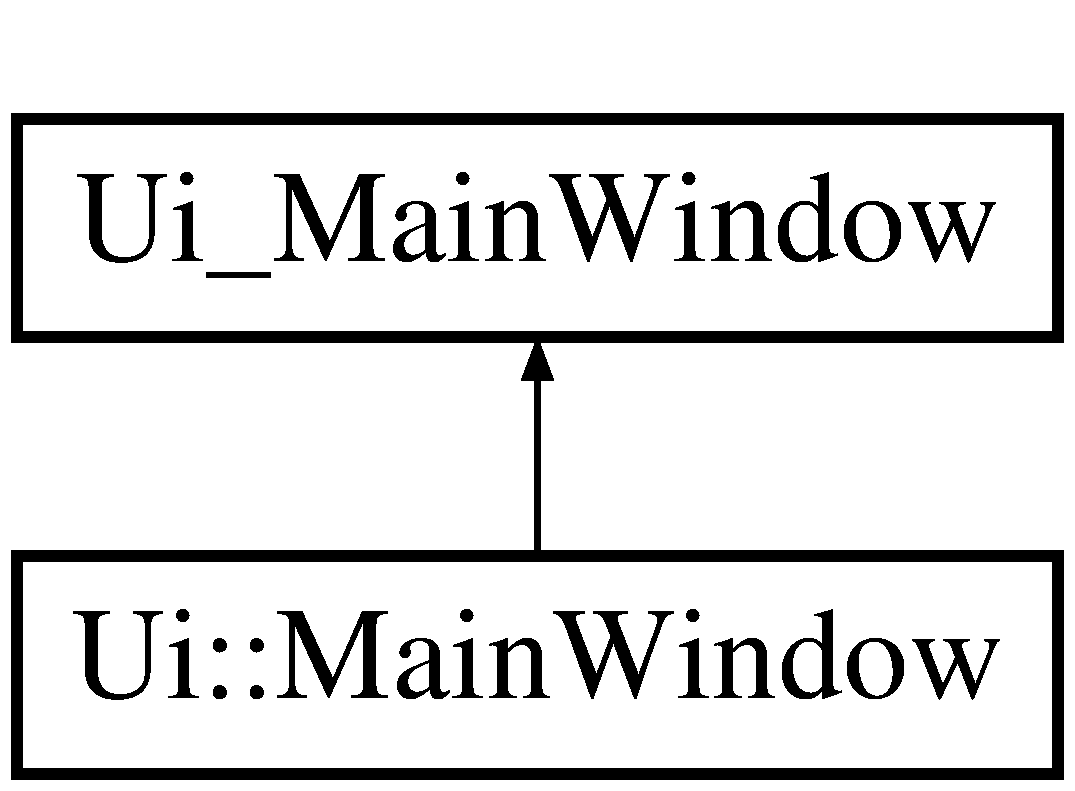
\includegraphics[height=2.000000cm]{class_ui_1_1_main_window}
\end{center}
\end{figure}
\subsection*{Additional Inherited Members}


The documentation for this class was generated from the following file\+:\begin{DoxyCompactItemize}
\item 
ui\+\_\+mainwindow.\+h\end{DoxyCompactItemize}

\hypertarget{structqt__meta__stringdata___export_wizard__t}{}\section{qt\+\_\+meta\+\_\+stringdata\+\_\+\+Export\+Wizard\+\_\+t Struct Reference}
\label{structqt__meta__stringdata___export_wizard__t}\index{qt\+\_\+meta\+\_\+stringdata\+\_\+\+Export\+Wizard\+\_\+t@{qt\+\_\+meta\+\_\+stringdata\+\_\+\+Export\+Wizard\+\_\+t}}
\subsection*{Public Attributes}
\begin{DoxyCompactItemize}
\item 
\hypertarget{structqt__meta__stringdata___export_wizard__t_a1c867d90aee99510b6673a23b1b54a57}{}Q\+Byte\+Array\+Data {\bfseries data} \mbox{[}3\mbox{]}\label{structqt__meta__stringdata___export_wizard__t_a1c867d90aee99510b6673a23b1b54a57}

\item 
\hypertarget{structqt__meta__stringdata___export_wizard__t_a7b6c20a6eb31458665043f44482ac81d}{}char {\bfseries stringdata0} \mbox{[}23\mbox{]}\label{structqt__meta__stringdata___export_wizard__t_a7b6c20a6eb31458665043f44482ac81d}

\end{DoxyCompactItemize}


The documentation for this struct was generated from the following file\+:\begin{DoxyCompactItemize}
\item 
moc\+\_\+exportwizard.\+cpp\end{DoxyCompactItemize}

\hypertarget{structqt__meta__stringdata___gantt_flow__t}{}\section{qt\+\_\+meta\+\_\+stringdata\+\_\+\+Gantt\+Flow\+\_\+t Struct Reference}
\label{structqt__meta__stringdata___gantt_flow__t}\index{qt\+\_\+meta\+\_\+stringdata\+\_\+\+Gantt\+Flow\+\_\+t@{qt\+\_\+meta\+\_\+stringdata\+\_\+\+Gantt\+Flow\+\_\+t}}
\subsection*{Public Attributes}
\begin{DoxyCompactItemize}
\item 
\hypertarget{structqt__meta__stringdata___gantt_flow__t_a8116996fb3a46fad828986cef0447fb6}{}Q\+Byte\+Array\+Data {\bfseries data} \mbox{[}4\mbox{]}\label{structqt__meta__stringdata___gantt_flow__t_a8116996fb3a46fad828986cef0447fb6}

\item 
\hypertarget{structqt__meta__stringdata___gantt_flow__t_aa1f6294d12182c1458eba7fdbb25736b}{}char {\bfseries stringdata0} \mbox{[}29\mbox{]}\label{structqt__meta__stringdata___gantt_flow__t_aa1f6294d12182c1458eba7fdbb25736b}

\end{DoxyCompactItemize}


The documentation for this struct was generated from the following file\+:\begin{DoxyCompactItemize}
\item 
moc\+\_\+ganttflow.\+cpp\end{DoxyCompactItemize}

\hypertarget{structqt__meta__stringdata___gantt_line__t}{}\section{qt\+\_\+meta\+\_\+stringdata\+\_\+\+Gantt\+Line\+\_\+t Struct Reference}
\label{structqt__meta__stringdata___gantt_line__t}\index{qt\+\_\+meta\+\_\+stringdata\+\_\+\+Gantt\+Line\+\_\+t@{qt\+\_\+meta\+\_\+stringdata\+\_\+\+Gantt\+Line\+\_\+t}}
\subsection*{Public Attributes}
\begin{DoxyCompactItemize}
\item 
\hypertarget{structqt__meta__stringdata___gantt_line__t_ae0a5d1655913c2dbadc51f0f5c2b0304}{}Q\+Byte\+Array\+Data {\bfseries data} \mbox{[}4\mbox{]}\label{structqt__meta__stringdata___gantt_line__t_ae0a5d1655913c2dbadc51f0f5c2b0304}

\item 
\hypertarget{structqt__meta__stringdata___gantt_line__t_aa375e7dd8d0e003680101fdca1f8492d}{}char {\bfseries stringdata0} \mbox{[}29\mbox{]}\label{structqt__meta__stringdata___gantt_line__t_aa375e7dd8d0e003680101fdca1f8492d}

\end{DoxyCompactItemize}


The documentation for this struct was generated from the following file\+:\begin{DoxyCompactItemize}
\item 
moc\+\_\+ganttline.\+cpp\end{DoxyCompactItemize}

\hypertarget{structqt__meta__stringdata___gantt_rect__t}{}\section{qt\+\_\+meta\+\_\+stringdata\+\_\+\+Gantt\+Rect\+\_\+t Struct Reference}
\label{structqt__meta__stringdata___gantt_rect__t}\index{qt\+\_\+meta\+\_\+stringdata\+\_\+\+Gantt\+Rect\+\_\+t@{qt\+\_\+meta\+\_\+stringdata\+\_\+\+Gantt\+Rect\+\_\+t}}
\subsection*{Public Attributes}
\begin{DoxyCompactItemize}
\item 
\hypertarget{structqt__meta__stringdata___gantt_rect__t_a57b6f9eed876c9b7314dadce4917a05c}{}Q\+Byte\+Array\+Data {\bfseries data} \mbox{[}6\mbox{]}\label{structqt__meta__stringdata___gantt_rect__t_a57b6f9eed876c9b7314dadce4917a05c}

\item 
\hypertarget{structqt__meta__stringdata___gantt_rect__t_a87738a6c7d7266096859472fd64b34c6}{}char {\bfseries stringdata0} \mbox{[}51\mbox{]}\label{structqt__meta__stringdata___gantt_rect__t_a87738a6c7d7266096859472fd64b34c6}

\end{DoxyCompactItemize}


The documentation for this struct was generated from the following file\+:\begin{DoxyCompactItemize}
\item 
moc\+\_\+ganttrect.\+cpp\end{DoxyCompactItemize}

\hypertarget{structqt__meta__stringdata___main_window__t}{}\section{qt\+\_\+meta\+\_\+stringdata\+\_\+\+Main\+Window\+\_\+t Struct Reference}
\label{structqt__meta__stringdata___main_window__t}\index{qt\+\_\+meta\+\_\+stringdata\+\_\+\+Main\+Window\+\_\+t@{qt\+\_\+meta\+\_\+stringdata\+\_\+\+Main\+Window\+\_\+t}}
\subsection*{Public Attributes}
\begin{DoxyCompactItemize}
\item 
\hypertarget{structqt__meta__stringdata___main_window__t_a941524227fa9b5bb71719febe2fb3895}{}Q\+Byte\+Array\+Data {\bfseries data} \mbox{[}54\mbox{]}\label{structqt__meta__stringdata___main_window__t_a941524227fa9b5bb71719febe2fb3895}

\item 
\hypertarget{structqt__meta__stringdata___main_window__t_a90b764002a8589a8ae9bec63ad953ec9}{}char {\bfseries stringdata0} \mbox{[}577\mbox{]}\label{structqt__meta__stringdata___main_window__t_a90b764002a8589a8ae9bec63ad953ec9}

\end{DoxyCompactItemize}


The documentation for this struct was generated from the following file\+:\begin{DoxyCompactItemize}
\item 
moc\+\_\+mainwindow.\+cpp\end{DoxyCompactItemize}

\hypertarget{structqt__meta__stringdata___wizard__t}{}\section{qt\+\_\+meta\+\_\+stringdata\+\_\+\+Wizard\+\_\+t Struct Reference}
\label{structqt__meta__stringdata___wizard__t}\index{qt\+\_\+meta\+\_\+stringdata\+\_\+\+Wizard\+\_\+t@{qt\+\_\+meta\+\_\+stringdata\+\_\+\+Wizard\+\_\+t}}
\subsection*{Public Attributes}
\begin{DoxyCompactItemize}
\item 
\hypertarget{structqt__meta__stringdata___wizard__t_abacf3e0c4161e300662056e354f10ef6}{}Q\+Byte\+Array\+Data {\bfseries data} \mbox{[}22\mbox{]}\label{structqt__meta__stringdata___wizard__t_abacf3e0c4161e300662056e354f10ef6}

\item 
\hypertarget{structqt__meta__stringdata___wizard__t_ab580891115b098af2494f04b9633726c}{}char {\bfseries stringdata0} \mbox{[}199\mbox{]}\label{structqt__meta__stringdata___wizard__t_ab580891115b098af2494f04b9633726c}

\end{DoxyCompactItemize}


The documentation for this struct was generated from the following file\+:\begin{DoxyCompactItemize}
\item 
moc\+\_\+wizard.\+cpp\end{DoxyCompactItemize}

\hypertarget{class_q_table_widget_number_item}{}\section{Q\+Table\+Widget\+Number\+Item Class Reference}
\label{class_q_table_widget_number_item}\index{Q\+Table\+Widget\+Number\+Item@{Q\+Table\+Widget\+Number\+Item}}
Inheritance diagram for Q\+Table\+Widget\+Number\+Item\+:\begin{figure}[H]
\begin{center}
\leavevmode
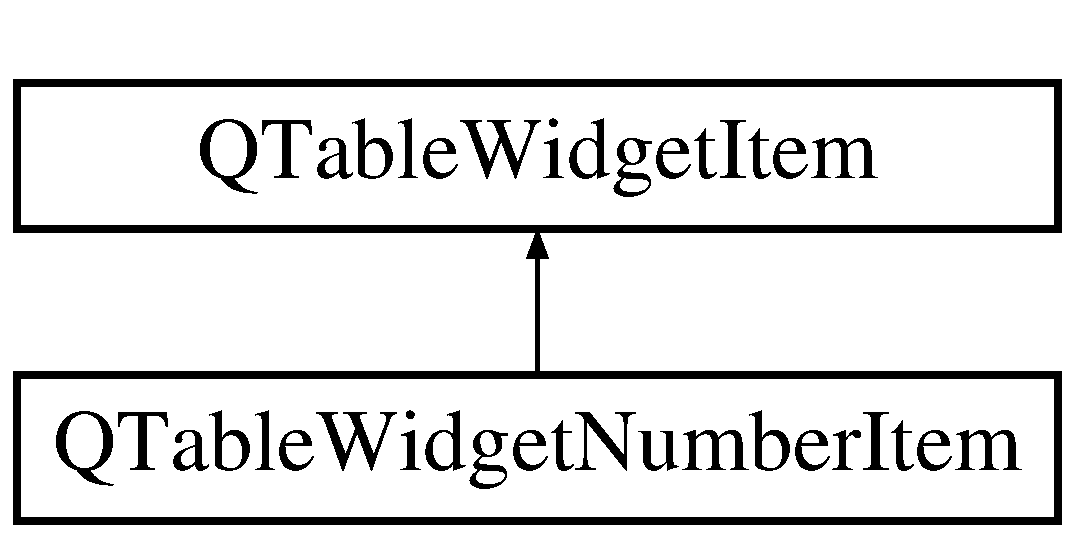
\includegraphics[height=2.000000cm]{class_q_table_widget_number_item}
\end{center}
\end{figure}
\subsection*{Public Member Functions}
\begin{DoxyCompactItemize}
\item 
\hypertarget{class_q_table_widget_number_item_af630e264aa968141468580baa4d34a64}{}{\bfseries Q\+Table\+Widget\+Number\+Item} (float number)\label{class_q_table_widget_number_item_af630e264aa968141468580baa4d34a64}

\item 
\hypertarget{class_q_table_widget_number_item_af788b33af492a04549f85a1b23a71c83}{}bool {\bfseries operator$<$} (const Q\+Table\+Widget\+Item \&other) const \label{class_q_table_widget_number_item_af788b33af492a04549f85a1b23a71c83}

\end{DoxyCompactItemize}


The documentation for this class was generated from the following files\+:\begin{DoxyCompactItemize}
\item 
qtablewidgetnumberitem.\+h\item 
qtablewidgetnumberitem.\+cpp\end{DoxyCompactItemize}

\hypertarget{struct_raw_flow}{}\section{Raw\+Flow Struct Reference}
\label{struct_raw_flow}\index{Raw\+Flow@{Raw\+Flow}}
\subsection*{Public Attributes}
\begin{DoxyCompactItemize}
\item 
\hypertarget{struct_raw_flow_a8a901b91a653344b5c1aa89b6b7aa146}{}float {\bfseries pr} = 0\label{struct_raw_flow_a8a901b91a653344b5c1aa89b6b7aa146}

\item 
\hypertarget{struct_raw_flow_ab43dc4259f2ce6a0e9767f7f2b2f7fad}{}float {\bfseries cr} = 0\label{struct_raw_flow_ab43dc4259f2ce6a0e9767f7f2b2f7fad}

\item 
\hypertarget{struct_raw_flow_ad3584703c40820da132e3a220182625b}{}float {\bfseries amount} = 0\label{struct_raw_flow_ad3584703c40820da132e3a220182625b}

\end{DoxyCompactItemize}


The documentation for this struct was generated from the following file\+:\begin{DoxyCompactItemize}
\item 
wizard.\+h\end{DoxyCompactItemize}

\hypertarget{struct_raw_task}{}\section{Raw\+Task Struct Reference}
\label{struct_raw_task}\index{Raw\+Task@{Raw\+Task}}
\subsection*{Public Attributes}
\begin{DoxyCompactItemize}
\item 
\hypertarget{struct_raw_task_aae3878eb2d74fac69fe87aafc1546da6}{}float {\bfseries start} = 0\label{struct_raw_task_aae3878eb2d74fac69fe87aafc1546da6}

\item 
\hypertarget{struct_raw_task_ae2a084841f755a15ce2cd7309d071729}{}float {\bfseries end} = 0\label{struct_raw_task_ae2a084841f755a15ce2cd7309d071729}

\item 
\hypertarget{struct_raw_task_ade899d7cdf5b71e5fbcd84097c9d052b}{}float {\bfseries amount} = 0\label{struct_raw_task_ade899d7cdf5b71e5fbcd84097c9d052b}

\item 
\hypertarget{struct_raw_task_ae0f990fca6dcf409ae62ccfb69616c99}{}float {\bfseries color} = -\/1\label{struct_raw_task_ae0f990fca6dcf409ae62ccfb69616c99}

\end{DoxyCompactItemize}


The documentation for this struct was generated from the following file\+:\begin{DoxyCompactItemize}
\item 
wizard.\+h\end{DoxyCompactItemize}

\hypertarget{struct_task}{}\section{Task Struct Reference}
\label{struct_task}\index{Task@{Task}}


representation of a task  




{\ttfamily \#include $<$mainwindow.\+h$>$}

\subsection*{Public Attributes}
\begin{DoxyCompactItemize}
\item 
\hypertarget{struct_task_a309b1c21e5d2ac19c5ed3c20bb2aa157}{}Q\+String \hyperlink{struct_task_a309b1c21e5d2ac19c5ed3c20bb2aa157}{name}\label{struct_task_a309b1c21e5d2ac19c5ed3c20bb2aa157}

\begin{DoxyCompactList}\small\item\em \hyperlink{struct_task}{Task} name. \end{DoxyCompactList}\item 
\hypertarget{struct_task_a39948d136b05540e7ad6dd1574e698a3}{}int \hyperlink{struct_task_a39948d136b05540e7ad6dd1574e698a3}{unit\+Index}\label{struct_task_a39948d136b05540e7ad6dd1574e698a3}

\begin{DoxyCompactList}\small\item\em The index of the unit the \hyperlink{struct_task}{Task} is on, in the \hyperlink{class_main_window_aad7505c53a0ad219080b3c1b1d1ef1e6}{Main\+Window\+::units} list. \end{DoxyCompactList}\item 
\hypertarget{struct_task_a57c58377752649d07774496b713a3b62}{}int \hyperlink{struct_task_a57c58377752649d07774496b713a3b62}{task\+Index}\label{struct_task_a57c58377752649d07774496b713a3b62}

\begin{DoxyCompactList}\small\item\em The index of this task in the \hyperlink{class_main_window_ab302362b256360d527a628bdbfcde171}{Main\+Window\+::tasks} list. \end{DoxyCompactList}\item 
\hypertarget{struct_task_aeec61bc8f3ff22ea69e6fe24723211f1}{}float \hyperlink{struct_task_aeec61bc8f3ff22ea69e6fe24723211f1}{start}\label{struct_task_aeec61bc8f3ff22ea69e6fe24723211f1}

\begin{DoxyCompactList}\small\item\em \hyperlink{struct_task}{Task} start time. \end{DoxyCompactList}\item 
\hypertarget{struct_task_a06201963cfc33c4efa69ba0321f96ae3}{}float \hyperlink{struct_task_a06201963cfc33c4efa69ba0321f96ae3}{end}\label{struct_task_a06201963cfc33c4efa69ba0321f96ae3}

\begin{DoxyCompactList}\small\item\em \hyperlink{struct_task}{Task} end time. \end{DoxyCompactList}\item 
\hypertarget{struct_task_a5969422039af2c60268de4df34018a92}{}float \hyperlink{struct_task_a5969422039af2c60268de4df34018a92}{amount}\label{struct_task_a5969422039af2c60268de4df34018a92}

\begin{DoxyCompactList}\small\item\em \hyperlink{struct_task}{Task} amount. \end{DoxyCompactList}\item 
\hypertarget{struct_task_a2f697912e846f50b1719bcc8dece716b}{}Q\+Color \hyperlink{struct_task_a2f697912e846f50b1719bcc8dece716b}{color}\label{struct_task_a2f697912e846f50b1719bcc8dece716b}

\begin{DoxyCompactList}\small\item\em The color of this task as defined in the input file. If no color is given, this will be set to a random color in \hyperlink{class_main_window_a2920d5c6c64925cb5f87c7fdac3f54b0}{Main\+Window\+::add\+Task}. \end{DoxyCompactList}\end{DoxyCompactItemize}


\subsection{Detailed Description}
representation of a task 

The documentation for this struct was generated from the following file\+:\begin{DoxyCompactItemize}
\item 
mainwindow.\+h\end{DoxyCompactItemize}

\hypertarget{class_ui___export_wizard}{}\section{Ui\+\_\+\+Export\+Wizard Class Reference}
\label{class_ui___export_wizard}\index{Ui\+\_\+\+Export\+Wizard@{Ui\+\_\+\+Export\+Wizard}}
Inheritance diagram for Ui\+\_\+\+Export\+Wizard\+:\begin{figure}[H]
\begin{center}
\leavevmode
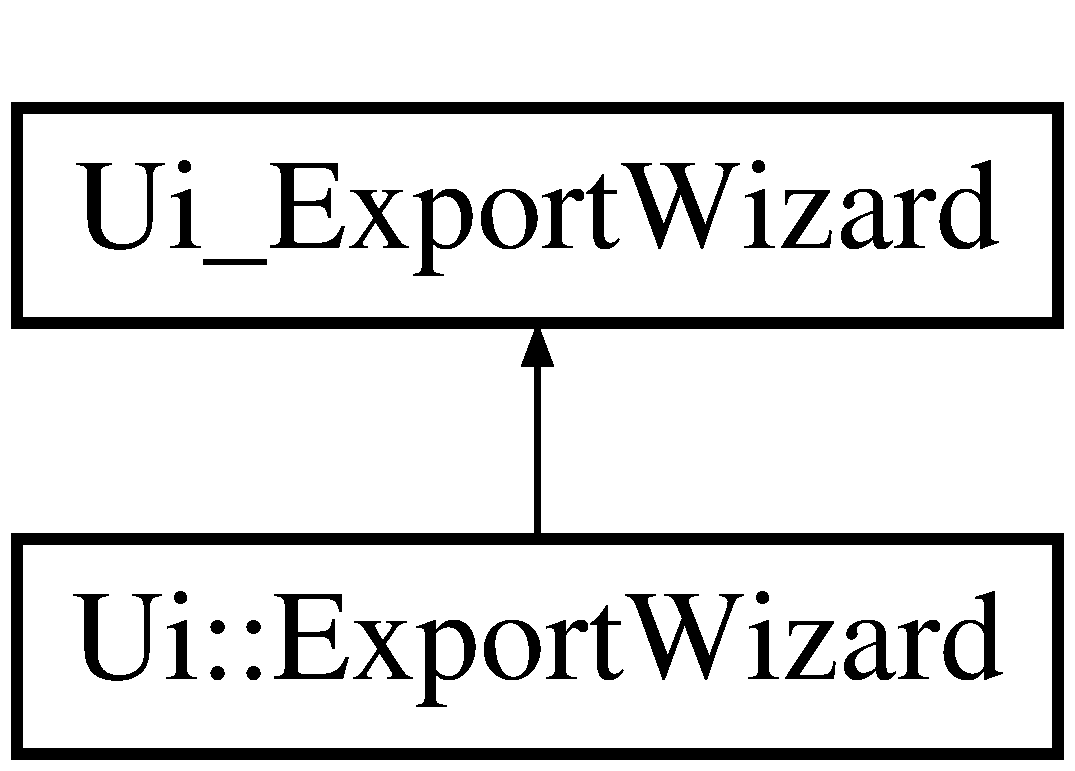
\includegraphics[height=2.000000cm]{class_ui___export_wizard}
\end{center}
\end{figure}
\subsection*{Public Member Functions}
\begin{DoxyCompactItemize}
\item 
\hypertarget{class_ui___export_wizard_aeb617b4b1c2c57a797a17552f6a2a336}{}void {\bfseries setup\+Ui} (Q\+Wizard $\ast$\hyperlink{class_export_wizard}{Export\+Wizard})\label{class_ui___export_wizard_aeb617b4b1c2c57a797a17552f6a2a336}

\item 
\hypertarget{class_ui___export_wizard_ae48fdbd6514577abbaa201f9d47c324d}{}void {\bfseries retranslate\+Ui} (Q\+Wizard $\ast$\hyperlink{class_export_wizard}{Export\+Wizard})\label{class_ui___export_wizard_ae48fdbd6514577abbaa201f9d47c324d}

\end{DoxyCompactItemize}
\subsection*{Public Attributes}
\begin{DoxyCompactItemize}
\item 
\hypertarget{class_ui___export_wizard_a947f9618e668529e07f3134debfb03ec}{}Q\+Wizard\+Page $\ast$ {\bfseries wizard\+Page1}\label{class_ui___export_wizard_a947f9618e668529e07f3134debfb03ec}

\item 
\hypertarget{class_ui___export_wizard_adf5c6138124efc5222a9b6c459f5eaef}{}Q\+Grid\+Layout $\ast$ {\bfseries grid\+Layout}\label{class_ui___export_wizard_adf5c6138124efc5222a9b6c459f5eaef}

\item 
\hypertarget{class_ui___export_wizard_a535c4dddfefd242b2513ba6d0fca3fdf}{}Q\+Label $\ast$ {\bfseries label}\label{class_ui___export_wizard_a535c4dddfefd242b2513ba6d0fca3fdf}

\item 
\hypertarget{class_ui___export_wizard_a36bde3332c52b3af4a247a80cf3bd7cc}{}Q\+Label $\ast$ {\bfseries label\+\_\+3}\label{class_ui___export_wizard_a36bde3332c52b3af4a247a80cf3bd7cc}

\item 
\hypertarget{class_ui___export_wizard_a1a6f444c4b34bf8918e75a708aca9a48}{}Q\+Check\+Box $\ast$ {\bfseries allflows}\label{class_ui___export_wizard_a1a6f444c4b34bf8918e75a708aca9a48}

\item 
\hypertarget{class_ui___export_wizard_ad0ccd5c8ee00945929af0db32630b0e3}{}Q\+Double\+Spin\+Box $\ast$ {\bfseries vscale}\label{class_ui___export_wizard_ad0ccd5c8ee00945929af0db32630b0e3}

\item 
\hypertarget{class_ui___export_wizard_abce9995832c7125157c9245e758f654f}{}Q\+Check\+Box $\ast$ {\bfseries labels}\label{class_ui___export_wizard_abce9995832c7125157c9245e758f654f}

\item 
\hypertarget{class_ui___export_wizard_afe818ed5624b88bb6fbfeae138a70d06}{}Q\+Combo\+Box $\ast$ {\bfseries color}\label{class_ui___export_wizard_afe818ed5624b88bb6fbfeae138a70d06}

\item 
\hypertarget{class_ui___export_wizard_a5a5b7e45e9c744c11ecf7eaf745f05a7}{}Q\+Combo\+Box $\ast$ {\bfseries format}\label{class_ui___export_wizard_a5a5b7e45e9c744c11ecf7eaf745f05a7}

\item 
\hypertarget{class_ui___export_wizard_a76cd23500ca5297b24b223d2e621505b}{}Q\+Label $\ast$ {\bfseries label\+\_\+2}\label{class_ui___export_wizard_a76cd23500ca5297b24b223d2e621505b}

\item 
\hypertarget{class_ui___export_wizard_a82ef8a2c3c6442f97f87a6ffe867fe8d}{}Q\+Check\+Box $\ast$ {\bfseries filter}\label{class_ui___export_wizard_a82ef8a2c3c6442f97f87a6ffe867fe8d}

\item 
\hypertarget{class_ui___export_wizard_a4fe8bd1f3aa9afbabad7b72a13601514}{}Q\+Label $\ast$ {\bfseries label\+\_\+4}\label{class_ui___export_wizard_a4fe8bd1f3aa9afbabad7b72a13601514}

\item 
\hypertarget{class_ui___export_wizard_aa5c1133dd13b25d208a93e3d19603b07}{}Q\+Spin\+Box $\ast$ {\bfseries interval}\label{class_ui___export_wizard_aa5c1133dd13b25d208a93e3d19603b07}

\end{DoxyCompactItemize}


The documentation for this class was generated from the following file\+:\begin{DoxyCompactItemize}
\item 
ui\+\_\+exportwizard.\+h\end{DoxyCompactItemize}

\hypertarget{class_ui___main_window}{}\section{Ui\+\_\+\+Main\+Window Class Reference}
\label{class_ui___main_window}\index{Ui\+\_\+\+Main\+Window@{Ui\+\_\+\+Main\+Window}}
Inheritance diagram for Ui\+\_\+\+Main\+Window\+:\begin{figure}[H]
\begin{center}
\leavevmode
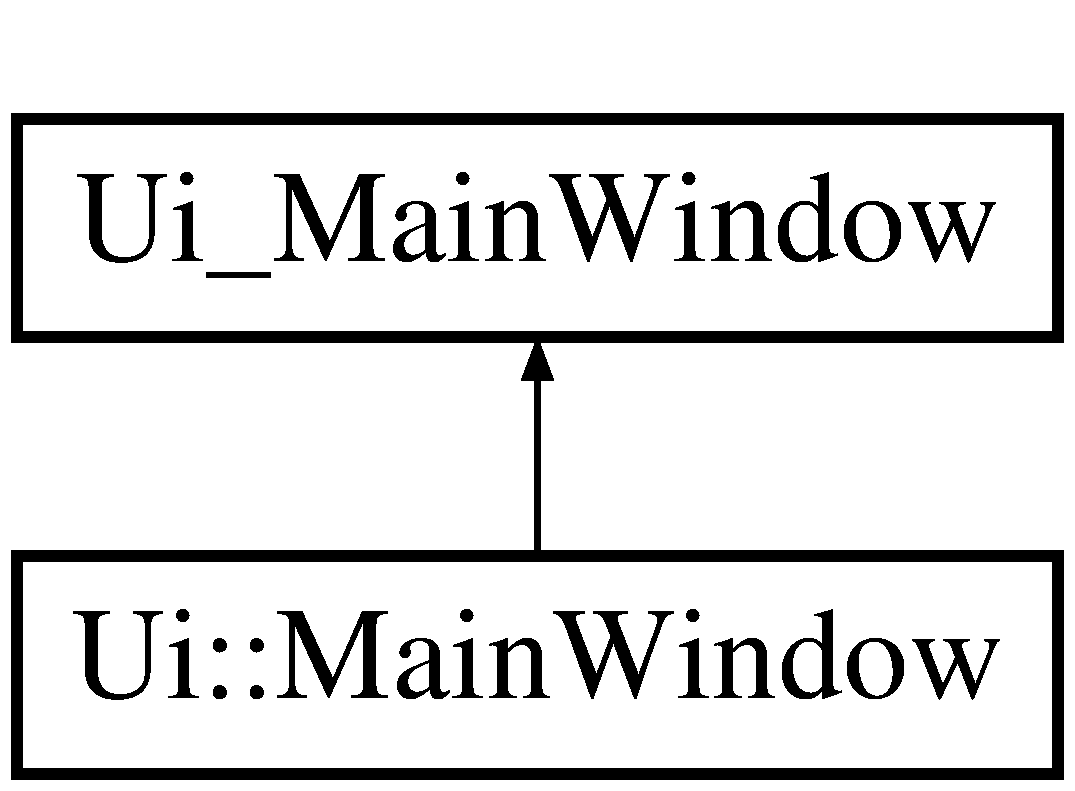
\includegraphics[height=2.000000cm]{class_ui___main_window}
\end{center}
\end{figure}
\subsection*{Public Member Functions}
\begin{DoxyCompactItemize}
\item 
\hypertarget{class_ui___main_window_acf4a0872c4c77d8f43a2ec66ed849b58}{}void {\bfseries setup\+Ui} (Q\+Main\+Window $\ast$\hyperlink{class_main_window}{Main\+Window})\label{class_ui___main_window_acf4a0872c4c77d8f43a2ec66ed849b58}

\item 
\hypertarget{class_ui___main_window_a097dd160c3534a204904cb374412c618}{}void {\bfseries retranslate\+Ui} (Q\+Main\+Window $\ast$\hyperlink{class_main_window}{Main\+Window})\label{class_ui___main_window_a097dd160c3534a204904cb374412c618}

\end{DoxyCompactItemize}
\subsection*{Public Attributes}
\begin{DoxyCompactItemize}
\item 
\hypertarget{class_ui___main_window_a30075506c2116c3ed4ff25e07ae75f81}{}Q\+Widget $\ast$ {\bfseries central\+Widget}\label{class_ui___main_window_a30075506c2116c3ed4ff25e07ae75f81}

\item 
\hypertarget{class_ui___main_window_a8ee86315639f324b17708efc7dbe8b19}{}Q\+Grid\+Layout $\ast$ {\bfseries grid\+Layout\+\_\+4}\label{class_ui___main_window_a8ee86315639f324b17708efc7dbe8b19}

\item 
\hypertarget{class_ui___main_window_af42ea7d4c2e893181caad21e28166932}{}Q\+Grid\+Layout $\ast$ {\bfseries grid\+Layout\+\_\+3}\label{class_ui___main_window_af42ea7d4c2e893181caad21e28166932}

\item 
\hypertarget{class_ui___main_window_acd6fdc9ebacc4b25b834162380d75ce8}{}Q\+H\+Box\+Layout $\ast$ {\bfseries horizontal\+Layout}\label{class_ui___main_window_acd6fdc9ebacc4b25b834162380d75ce8}

\item 
\hypertarget{class_ui___main_window_adb342c5978b7d4791294faa8aab5683c}{}Q\+Push\+Button $\ast$ {\bfseries toggle\+Button}\label{class_ui___main_window_adb342c5978b7d4791294faa8aab5683c}

\item 
\hypertarget{class_ui___main_window_a2e2516d755e4dd53fc905dabddf2738a}{}Q\+Label $\ast$ {\bfseries label\+\_\+2}\label{class_ui___main_window_a2e2516d755e4dd53fc905dabddf2738a}

\item 
\hypertarget{class_ui___main_window_a5c4fff8d6ea22c9e3e403d1af9c36b26}{}Q\+Push\+Button $\ast$ {\bfseries v\+\_\+zoom\+\_\+out}\label{class_ui___main_window_a5c4fff8d6ea22c9e3e403d1af9c36b26}

\item 
\hypertarget{class_ui___main_window_acc5d089772e8cdc8c53b20e42b7d80bc}{}Q\+Slider $\ast$ {\bfseries vertical\+Slider}\label{class_ui___main_window_acc5d089772e8cdc8c53b20e42b7d80bc}

\item 
\hypertarget{class_ui___main_window_a4c2ce998deb05bc0719d89d37215596e}{}Q\+Push\+Button $\ast$ {\bfseries v\+\_\+zoom\+\_\+in}\label{class_ui___main_window_a4c2ce998deb05bc0719d89d37215596e}

\item 
\hypertarget{class_ui___main_window_ad9c89133780f28e6efa2ec17ceb9cff5}{}Q\+Label $\ast$ {\bfseries label}\label{class_ui___main_window_ad9c89133780f28e6efa2ec17ceb9cff5}

\item 
\hypertarget{class_ui___main_window_a678ab335af4149516e91783e4007a0fc}{}Q\+Push\+Button $\ast$ {\bfseries h\+\_\+zoom\+\_\+out}\label{class_ui___main_window_a678ab335af4149516e91783e4007a0fc}

\item 
\hypertarget{class_ui___main_window_ae0d25af9b3ed9386441e76f06d3f3ddb}{}Q\+Slider $\ast$ {\bfseries horizontal\+Slider}\label{class_ui___main_window_ae0d25af9b3ed9386441e76f06d3f3ddb}

\item 
\hypertarget{class_ui___main_window_afe725d9fc9be76f799729b00aaa6e7ef}{}Q\+Push\+Button $\ast$ {\bfseries h\+\_\+zoom\+\_\+in}\label{class_ui___main_window_afe725d9fc9be76f799729b00aaa6e7ef}

\item 
\hypertarget{class_ui___main_window_a32580a08aa05697cc452a271a20adbea}{}Q\+Push\+Button $\ast$ {\bfseries center\+Button}\label{class_ui___main_window_a32580a08aa05697cc452a271a20adbea}

\item 
\hypertarget{class_ui___main_window_abfba98fab6f5677d35fa69dd46ef8ffb}{}Q\+Splitter $\ast$ {\bfseries splitter}\label{class_ui___main_window_abfba98fab6f5677d35fa69dd46ef8ffb}

\item 
\hypertarget{class_ui___main_window_ab96ab0f0578098521fa69a75aa5cdde8}{}Q\+Widget $\ast$ {\bfseries layout\+Widget}\label{class_ui___main_window_ab96ab0f0578098521fa69a75aa5cdde8}

\item 
\hypertarget{class_ui___main_window_a411e815aa62387a693c1ffd0340219f6}{}Q\+V\+Box\+Layout $\ast$ {\bfseries Sidebar}\label{class_ui___main_window_a411e815aa62387a693c1ffd0340219f6}

\item 
\hypertarget{class_ui___main_window_a337a21c052f1a3f0f0071d282e818744}{}Q\+Table\+Widget $\ast$ {\bfseries table\+Widget}\label{class_ui___main_window_a337a21c052f1a3f0f0071d282e818744}

\item 
\hypertarget{class_ui___main_window_a3260b943854b841c986f47c4726ee7f9}{}Q\+Tab\+Widget $\ast$ {\bfseries tab\+Widget}\label{class_ui___main_window_a3260b943854b841c986f47c4726ee7f9}

\item 
\hypertarget{class_ui___main_window_a746d3ea94f2f6de494bab86b5bedbe45}{}Q\+Widget $\ast$ {\bfseries tasks\+Tab}\label{class_ui___main_window_a746d3ea94f2f6de494bab86b5bedbe45}

\item 
\hypertarget{class_ui___main_window_a0c01bad60d9f422a1258e710635a2f65}{}Q\+V\+Box\+Layout $\ast$ {\bfseries vertical\+Layout\+\_\+2}\label{class_ui___main_window_a0c01bad60d9f422a1258e710635a2f65}

\item 
\hypertarget{class_ui___main_window_a5b2d9adfb766a8c34095c77fdbb01308}{}Q\+Table\+Widget $\ast$ {\bfseries all\+Tasks\+Table}\label{class_ui___main_window_a5b2d9adfb766a8c34095c77fdbb01308}

\item 
\hypertarget{class_ui___main_window_a48309390837887aa5ca2b75efbbe3dff}{}Q\+Widget $\ast$ {\bfseries filter\+Tab}\label{class_ui___main_window_a48309390837887aa5ca2b75efbbe3dff}

\item 
\hypertarget{class_ui___main_window_a525ed3c5fe0784ac502ee222fba4e205}{}Q\+Grid\+Layout $\ast$ {\bfseries grid\+Layout}\label{class_ui___main_window_a525ed3c5fe0784ac502ee222fba4e205}

\item 
\hypertarget{class_ui___main_window_ad6bab8fb8903b8f41afea1218ee52695}{}Q\+Label $\ast$ {\bfseries label\+\_\+5}\label{class_ui___main_window_ad6bab8fb8903b8f41afea1218ee52695}

\item 
\hypertarget{class_ui___main_window_a663f728e6244926a795c6e6892673b1d}{}Q\+Label $\ast$ {\bfseries label\+\_\+6}\label{class_ui___main_window_a663f728e6244926a795c6e6892673b1d}

\item 
\hypertarget{class_ui___main_window_ad192feddb3fdc3d2dcacd21fa9c41e5d}{}Q\+Double\+Spin\+Box $\ast$ {\bfseries filter1start}\label{class_ui___main_window_ad192feddb3fdc3d2dcacd21fa9c41e5d}

\item 
\hypertarget{class_ui___main_window_a871c836255fa8638d185a4dc66f1ae92}{}Q\+Line\+Edit $\ast$ {\bfseries filter\+Task}\label{class_ui___main_window_a871c836255fa8638d185a4dc66f1ae92}

\item 
\hypertarget{class_ui___main_window_adca5dfd2c6ed2e19c63950e9eb5444d0}{}Q\+Double\+Spin\+Box $\ast$ {\bfseries filter2end}\label{class_ui___main_window_adca5dfd2c6ed2e19c63950e9eb5444d0}

\item 
\hypertarget{class_ui___main_window_aa7db1aafba27c67bb4f179b1986ed7dd}{}Q\+Combo\+Box $\ast$ {\bfseries rule\+End}\label{class_ui___main_window_aa7db1aafba27c67bb4f179b1986ed7dd}

\item 
\hypertarget{class_ui___main_window_af183bfbfb9f38bbdd60caf92b15e23dc}{}Q\+Label $\ast$ {\bfseries label\+\_\+8}\label{class_ui___main_window_af183bfbfb9f38bbdd60caf92b15e23dc}

\item 
\hypertarget{class_ui___main_window_a0a9a603174c0f6617cf48bbf74342c52}{}Q\+Double\+Spin\+Box $\ast$ {\bfseries filter2duration}\label{class_ui___main_window_a0a9a603174c0f6617cf48bbf74342c52}

\item 
\hypertarget{class_ui___main_window_a60a44a160823bc50ce08deac1a0f44b1}{}Q\+Double\+Spin\+Box $\ast$ {\bfseries filter2start}\label{class_ui___main_window_a60a44a160823bc50ce08deac1a0f44b1}

\item 
\hypertarget{class_ui___main_window_ad2f8c232d831e44219b71798dcc72ab4}{}Q\+Double\+Spin\+Box $\ast$ {\bfseries filter1amount}\label{class_ui___main_window_ad2f8c232d831e44219b71798dcc72ab4}

\item 
\hypertarget{class_ui___main_window_a85bf5794801d0ef195874b001472b0d7}{}Q\+Double\+Spin\+Box $\ast$ {\bfseries filter2amount}\label{class_ui___main_window_a85bf5794801d0ef195874b001472b0d7}

\item 
\hypertarget{class_ui___main_window_a6559f3b9fc30f43e56cb3df974bf39c4}{}Q\+Double\+Spin\+Box $\ast$ {\bfseries filter1duration}\label{class_ui___main_window_a6559f3b9fc30f43e56cb3df974bf39c4}

\item 
\hypertarget{class_ui___main_window_aa197044096a72b1e2d3b0f5cbc6ff118}{}Q\+Combo\+Box $\ast$ {\bfseries rule\+Start}\label{class_ui___main_window_aa197044096a72b1e2d3b0f5cbc6ff118}

\item 
\hypertarget{class_ui___main_window_a78c7e10730b43c6700cd7216911ed76a}{}Q\+Label $\ast$ {\bfseries label\+\_\+4}\label{class_ui___main_window_a78c7e10730b43c6700cd7216911ed76a}

\item 
\hypertarget{class_ui___main_window_a2389f27e15b3a0c6a2db352c906c21e9}{}Q\+Line\+Edit $\ast$ {\bfseries filter\+Unit}\label{class_ui___main_window_a2389f27e15b3a0c6a2db352c906c21e9}

\item 
\hypertarget{class_ui___main_window_a8c00de6d559b805dc1a7159677a60f97}{}Q\+Double\+Spin\+Box $\ast$ {\bfseries filter1end}\label{class_ui___main_window_a8c00de6d559b805dc1a7159677a60f97}

\item 
\hypertarget{class_ui___main_window_a0e90c7e9ad77386881e0b264ddb9dd22}{}Q\+Label $\ast$ {\bfseries label\+\_\+9}\label{class_ui___main_window_a0e90c7e9ad77386881e0b264ddb9dd22}

\item 
\hypertarget{class_ui___main_window_ae4213edfe8328bb829075613e7c7043e}{}Q\+Combo\+Box $\ast$ {\bfseries rule\+Duration}\label{class_ui___main_window_ae4213edfe8328bb829075613e7c7043e}

\item 
\hypertarget{class_ui___main_window_a0376fd90247280e7c7957cc70628708c}{}Q\+Label $\ast$ {\bfseries label\+\_\+3}\label{class_ui___main_window_a0376fd90247280e7c7957cc70628708c}

\item 
\hypertarget{class_ui___main_window_a67366bae41eff3fe77753cffb11f19ac}{}Q\+Combo\+Box $\ast$ {\bfseries rule\+Amount}\label{class_ui___main_window_a67366bae41eff3fe77753cffb11f19ac}

\item 
\hypertarget{class_ui___main_window_a77f37bd7214815da06093db704ec8e55}{}Q\+Push\+Button $\ast$ {\bfseries filter\+Apply\+Button}\label{class_ui___main_window_a77f37bd7214815da06093db704ec8e55}

\item 
\hypertarget{class_ui___main_window_a6308d77991290fdc5381130325b6fcdd}{}Q\+Push\+Button $\ast$ {\bfseries filter\+Clear\+Button}\label{class_ui___main_window_a6308d77991290fdc5381130325b6fcdd}

\item 
\hypertarget{class_ui___main_window_a84cae8297d91efe5a48546c9e8874632}{}Q\+Label $\ast$ {\bfseries table\+Count}\label{class_ui___main_window_a84cae8297d91efe5a48546c9e8874632}

\item 
\hypertarget{class_ui___main_window_aa5baadb06f60aa8a57a9f7fe168d284a}{}Q\+Widget $\ast$ {\bfseries errors\+Tab}\label{class_ui___main_window_aa5baadb06f60aa8a57a9f7fe168d284a}

\item 
\hypertarget{class_ui___main_window_aecd96a04789fcfec3f98d80390ad8184}{}Q\+V\+Box\+Layout $\ast$ {\bfseries vertical\+Layout}\label{class_ui___main_window_aecd96a04789fcfec3f98d80390ad8184}

\item 
\hypertarget{class_ui___main_window_a7d8c07c464bdd9ae616d88d5d85f5c13}{}Q\+Text\+Browser $\ast$ {\bfseries errors\+Viewer}\label{class_ui___main_window_a7d8c07c464bdd9ae616d88d5d85f5c13}

\item 
\hypertarget{class_ui___main_window_a7f6b63ce7ca36d553480fc0b20b15b0e}{}Q\+Push\+Button $\ast$ {\bfseries save\+Button}\label{class_ui___main_window_a7f6b63ce7ca36d553480fc0b20b15b0e}

\item 
\hypertarget{class_ui___main_window_aab31b3dec8d767525dea6f163e029e48}{}Q\+Widget $\ast$ {\bfseries layout\+Widget1}\label{class_ui___main_window_aab31b3dec8d767525dea6f163e029e48}

\item 
\hypertarget{class_ui___main_window_a6b2a0c5f7e8ff2a87134908dd770d2d2}{}Q\+Grid\+Layout $\ast$ {\bfseries grid\+Layout\+\_\+2}\label{class_ui___main_window_a6b2a0c5f7e8ff2a87134908dd770d2d2}

\item 
\hypertarget{class_ui___main_window_a410197c6a086853ecb67b777a5d6eab1}{}Q\+Graphics\+View $\ast$ {\bfseries ruler\+View}\label{class_ui___main_window_a410197c6a086853ecb67b777a5d6eab1}

\item 
\hypertarget{class_ui___main_window_ad2d4f53301cf9cb6ecdb606e6bbbe9b2}{}Q\+Graphics\+View $\ast$ {\bfseries label\+View}\label{class_ui___main_window_ad2d4f53301cf9cb6ecdb606e6bbbe9b2}

\item 
\hypertarget{class_ui___main_window_a43a3a453d89302e0ba6101a82aacb1d0}{}Q\+Graphics\+View $\ast$ {\bfseries gantt\+View}\label{class_ui___main_window_a43a3a453d89302e0ba6101a82aacb1d0}

\item 
\hypertarget{class_ui___main_window_a5172877001c8c7b4e0f6de50421867d1}{}Q\+Tool\+Bar $\ast$ {\bfseries main\+Tool\+Bar}\label{class_ui___main_window_a5172877001c8c7b4e0f6de50421867d1}

\item 
\hypertarget{class_ui___main_window_a50fa481337604bcc8bf68de18ab16ecd}{}Q\+Status\+Bar $\ast$ {\bfseries status\+Bar}\label{class_ui___main_window_a50fa481337604bcc8bf68de18ab16ecd}

\item 
\hypertarget{class_ui___main_window_a2be1c24ec9adfca18e1dcc951931457f}{}Q\+Menu\+Bar $\ast$ {\bfseries menu\+Bar}\label{class_ui___main_window_a2be1c24ec9adfca18e1dcc951931457f}

\end{DoxyCompactItemize}


The documentation for this class was generated from the following file\+:\begin{DoxyCompactItemize}
\item 
ui\+\_\+mainwindow.\+h\end{DoxyCompactItemize}

\hypertarget{class_ui___wizard}{}\section{Ui\+\_\+\+Wizard Class Reference}
\label{class_ui___wizard}\index{Ui\+\_\+\+Wizard@{Ui\+\_\+\+Wizard}}
Inheritance diagram for Ui\+\_\+\+Wizard\+:\begin{figure}[H]
\begin{center}
\leavevmode
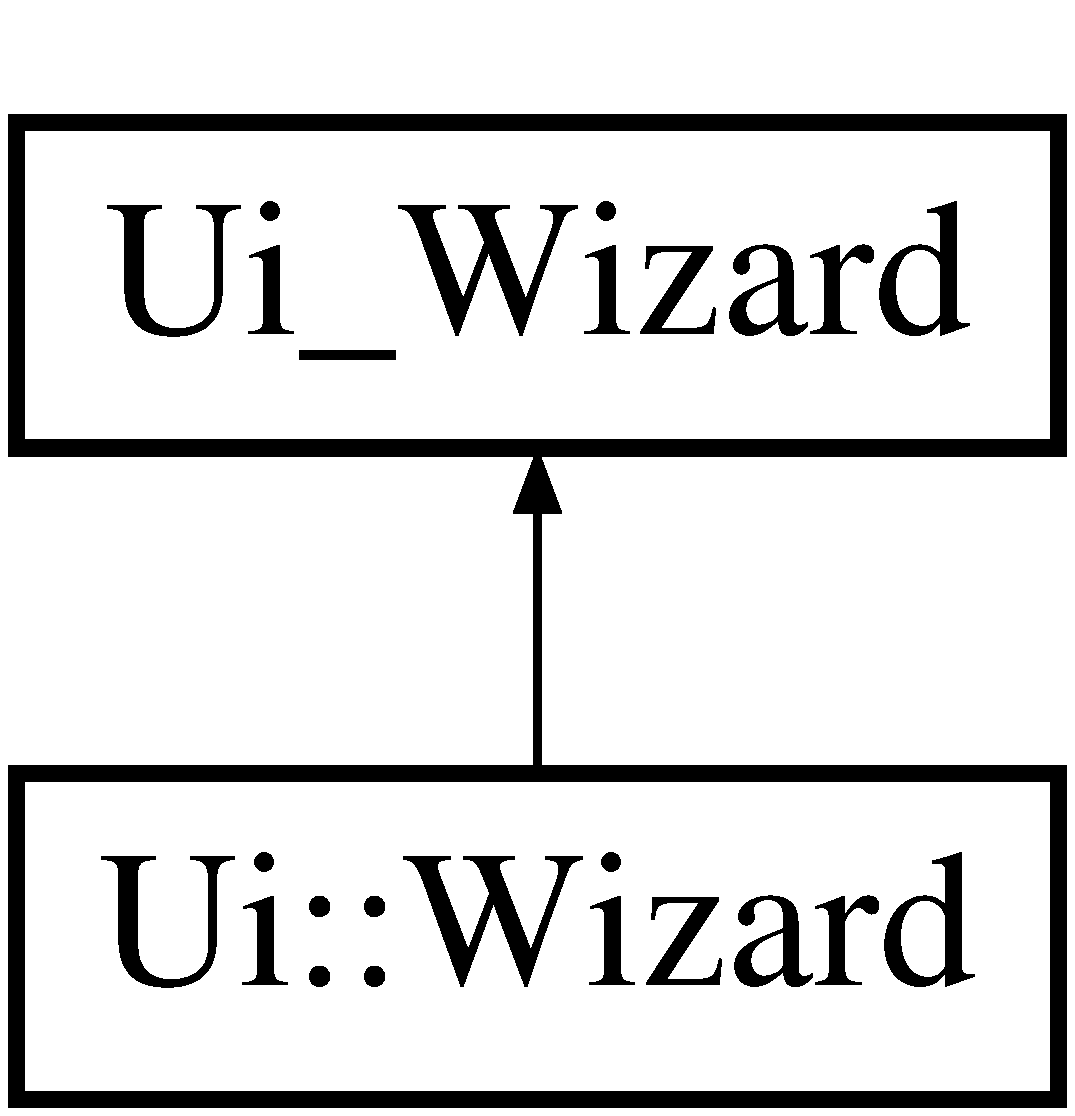
\includegraphics[height=2.000000cm]{class_ui___wizard}
\end{center}
\end{figure}
\subsection*{Public Member Functions}
\begin{DoxyCompactItemize}
\item 
\hypertarget{class_ui___wizard_a3da6248185e41358014012105bd59c56}{}void {\bfseries setup\+Ui} (Q\+Wizard $\ast$\hyperlink{class_wizard}{Wizard})\label{class_ui___wizard_a3da6248185e41358014012105bd59c56}

\item 
\hypertarget{class_ui___wizard_a123484236c302371968f46976bbdf2d7}{}void {\bfseries retranslate\+Ui} (Q\+Wizard $\ast$\hyperlink{class_wizard}{Wizard})\label{class_ui___wizard_a123484236c302371968f46976bbdf2d7}

\end{DoxyCompactItemize}
\subsection*{Public Attributes}
\begin{DoxyCompactItemize}
\item 
\hypertarget{class_ui___wizard_a593dd7776e690db14bc5d1978b2ca96f}{}Q\+Wizard\+Page $\ast$ {\bfseries wizard\+Page\+Load}\label{class_ui___wizard_a593dd7776e690db14bc5d1978b2ca96f}

\item 
\hypertarget{class_ui___wizard_ab8332309b854addbca78ed6dd9355381}{}Q\+Grid\+Layout $\ast$ {\bfseries grid\+Layout\+\_\+5}\label{class_ui___wizard_ab8332309b854addbca78ed6dd9355381}

\item 
\hypertarget{class_ui___wizard_a8a8caaa62eaac3b495975dae8dbd8a09}{}Q\+Label $\ast$ {\bfseries loaded\+File\+Label}\label{class_ui___wizard_a8a8caaa62eaac3b495975dae8dbd8a09}

\item 
\hypertarget{class_ui___wizard_a6805cbd003279c9e8e7b8f5a5b582356}{}Q\+Push\+Button $\ast$ {\bfseries load\+File\+Button}\label{class_ui___wizard_a6805cbd003279c9e8e7b8f5a5b582356}

\item 
\hypertarget{class_ui___wizard_a0bf86f996fa4297f08ca8cc681007474}{}Q\+Label $\ast$ {\bfseries loaded\+Config\+File\+Label}\label{class_ui___wizard_a0bf86f996fa4297f08ca8cc681007474}

\item 
\hypertarget{class_ui___wizard_abfe58822e5839d6c013418c08d05f718}{}Q\+Label $\ast$ {\bfseries sysdir\+Label}\label{class_ui___wizard_abfe58822e5839d6c013418c08d05f718}

\item 
\hypertarget{class_ui___wizard_a9dee27024353f55b77bd2e27f21abc0c}{}Q\+Push\+Button $\ast$ {\bfseries load\+Sysdir\+Button}\label{class_ui___wizard_a9dee27024353f55b77bd2e27f21abc0c}

\item 
\hypertarget{class_ui___wizard_a7f739a54ec930c446638a01bf14ff0be}{}Q\+Push\+Button $\ast$ {\bfseries load\+Config\+Button}\label{class_ui___wizard_a7f739a54ec930c446638a01bf14ff0be}

\item 
\hypertarget{class_ui___wizard_a0838e504fcf3d60d112fd695b8ad3687}{}Q\+Wizard\+Page $\ast$ {\bfseries wizard\+Page\+Tasks}\label{class_ui___wizard_a0838e504fcf3d60d112fd695b8ad3687}

\item 
\hypertarget{class_ui___wizard_af35f862ada391b88013d41f0d350f2d0}{}Q\+Grid\+Layout $\ast$ {\bfseries grid\+Layout}\label{class_ui___wizard_af35f862ada391b88013d41f0d350f2d0}

\item 
\hypertarget{class_ui___wizard_afe81db1eca97d8b3e86dac8d8d34ac4c}{}Q\+Grid\+Layout $\ast$ {\bfseries grid\+Layout\+\_\+2}\label{class_ui___wizard_afe81db1eca97d8b3e86dac8d8d34ac4c}

\item 
\hypertarget{class_ui___wizard_a4b380f70ab65745a4d2eaabbcae4344b}{}Q\+Label $\ast$ {\bfseries label\+\_\+3}\label{class_ui___wizard_a4b380f70ab65745a4d2eaabbcae4344b}

\item 
\hypertarget{class_ui___wizard_a6e054f0b887068437a7b18e384fbe493}{}Q\+Label $\ast$ {\bfseries label}\label{class_ui___wizard_a6e054f0b887068437a7b18e384fbe493}

\item 
\hypertarget{class_ui___wizard_a33b97f36885531b231c2807a8e4a0c4a}{}Q\+Label $\ast$ {\bfseries label\+\_\+2}\label{class_ui___wizard_a33b97f36885531b231c2807a8e4a0c4a}

\item 
\hypertarget{class_ui___wizard_a7546e9f661e838464a71afd731ec936d}{}Q\+Combo\+Box $\ast$ {\bfseries select\+Start}\label{class_ui___wizard_a7546e9f661e838464a71afd731ec936d}

\item 
\hypertarget{class_ui___wizard_a9ae3d871340717f09635bbc565b46b11}{}Q\+Label $\ast$ {\bfseries label\+\_\+4}\label{class_ui___wizard_a9ae3d871340717f09635bbc565b46b11}

\item 
\hypertarget{class_ui___wizard_a10ebcc4df6e1918faf2d0783a3b74c2e}{}Q\+Combo\+Box $\ast$ {\bfseries select\+End}\label{class_ui___wizard_a10ebcc4df6e1918faf2d0783a3b74c2e}

\item 
\hypertarget{class_ui___wizard_ac5f4f9619f99ec6727d1e9c897103ed4}{}Q\+Combo\+Box $\ast$ {\bfseries select\+Amount}\label{class_ui___wizard_ac5f4f9619f99ec6727d1e9c897103ed4}

\item 
\hypertarget{class_ui___wizard_ad97c295a57f9afac79acfe360d073eb3}{}Q\+Combo\+Box $\ast$ {\bfseries select\+Color}\label{class_ui___wizard_ad97c295a57f9afac79acfe360d073eb3}

\item 
\hypertarget{class_ui___wizard_af1d069be699c40606ebb28aafc115089}{}Q\+Wizard\+Page $\ast$ {\bfseries wizard\+Page\+Flows}\label{class_ui___wizard_af1d069be699c40606ebb28aafc115089}

\item 
\hypertarget{class_ui___wizard_a51d082e69bff333e80bbfeb37a52b37a}{}Q\+Grid\+Layout $\ast$ {\bfseries grid\+Layout\+\_\+4}\label{class_ui___wizard_a51d082e69bff333e80bbfeb37a52b37a}

\item 
\hypertarget{class_ui___wizard_a927647b5add8b6c1b79f11b4e1c59936}{}Q\+Grid\+Layout $\ast$ {\bfseries grid\+Layout\+\_\+3}\label{class_ui___wizard_a927647b5add8b6c1b79f11b4e1c59936}

\item 
\hypertarget{class_ui___wizard_a56e32ea802bb188b9d034f384a4daaaa}{}Q\+Label $\ast$ {\bfseries label\+\_\+5}\label{class_ui___wizard_a56e32ea802bb188b9d034f384a4daaaa}

\item 
\hypertarget{class_ui___wizard_ae9e58c61c868d1a26b5d4e116479780c}{}Q\+Label $\ast$ {\bfseries label\+\_\+6}\label{class_ui___wizard_ae9e58c61c868d1a26b5d4e116479780c}

\item 
\hypertarget{class_ui___wizard_ac777c566289cbf3f5c6fbbfb95afd488}{}Q\+Combo\+Box $\ast$ {\bfseries select\+Flow\+Amount}\label{class_ui___wizard_ac777c566289cbf3f5c6fbbfb95afd488}

\item 
\hypertarget{class_ui___wizard_ab4aa5ed390bb7487ce3eabeee821e324}{}Q\+Label $\ast$ {\bfseries label\+\_\+7}\label{class_ui___wizard_ab4aa5ed390bb7487ce3eabeee821e324}

\item 
\hypertarget{class_ui___wizard_a0ca027cde31ee5bd472eb56d5d301bbf}{}Q\+Combo\+Box $\ast$ {\bfseries select\+Pr}\label{class_ui___wizard_a0ca027cde31ee5bd472eb56d5d301bbf}

\item 
\hypertarget{class_ui___wizard_a237f8604727f7721dc8d51f089fd8d1a}{}Q\+Combo\+Box $\ast$ {\bfseries select\+Cr}\label{class_ui___wizard_a237f8604727f7721dc8d51f089fd8d1a}

\item 
\hypertarget{class_ui___wizard_aa156e1350b0158969c4acfc7fe0d0d63}{}Q\+Check\+Box $\ast$ {\bfseries check\+Box}\label{class_ui___wizard_aa156e1350b0158969c4acfc7fe0d0d63}

\item 
\hypertarget{class_ui___wizard_a569b85ea802d49f3becc1839f54c40b3}{}Q\+Wizard\+Page $\ast$ {\bfseries wizard\+Page\+Save\+Config}\label{class_ui___wizard_a569b85ea802d49f3becc1839f54c40b3}

\item 
\hypertarget{class_ui___wizard_a651da1d973c283d2234516c1e462c7b9}{}Q\+Form\+Layout $\ast$ {\bfseries form\+Layout}\label{class_ui___wizard_a651da1d973c283d2234516c1e462c7b9}

\item 
\hypertarget{class_ui___wizard_a59bd83391de9734acec79797a473a58f}{}Q\+Push\+Button $\ast$ {\bfseries save\+Config\+Button}\label{class_ui___wizard_a59bd83391de9734acec79797a473a58f}

\end{DoxyCompactItemize}


The documentation for this class was generated from the following file\+:\begin{DoxyCompactItemize}
\item 
ui\+\_\+wizard.\+h\end{DoxyCompactItemize}

\hypertarget{class_ui_1_1_wizard}{}\section{Ui\+:\+:Wizard Class Reference}
\label{class_ui_1_1_wizard}\index{Ui\+::\+Wizard@{Ui\+::\+Wizard}}
Inheritance diagram for Ui\+:\+:Wizard\+:\begin{figure}[H]
\begin{center}
\leavevmode
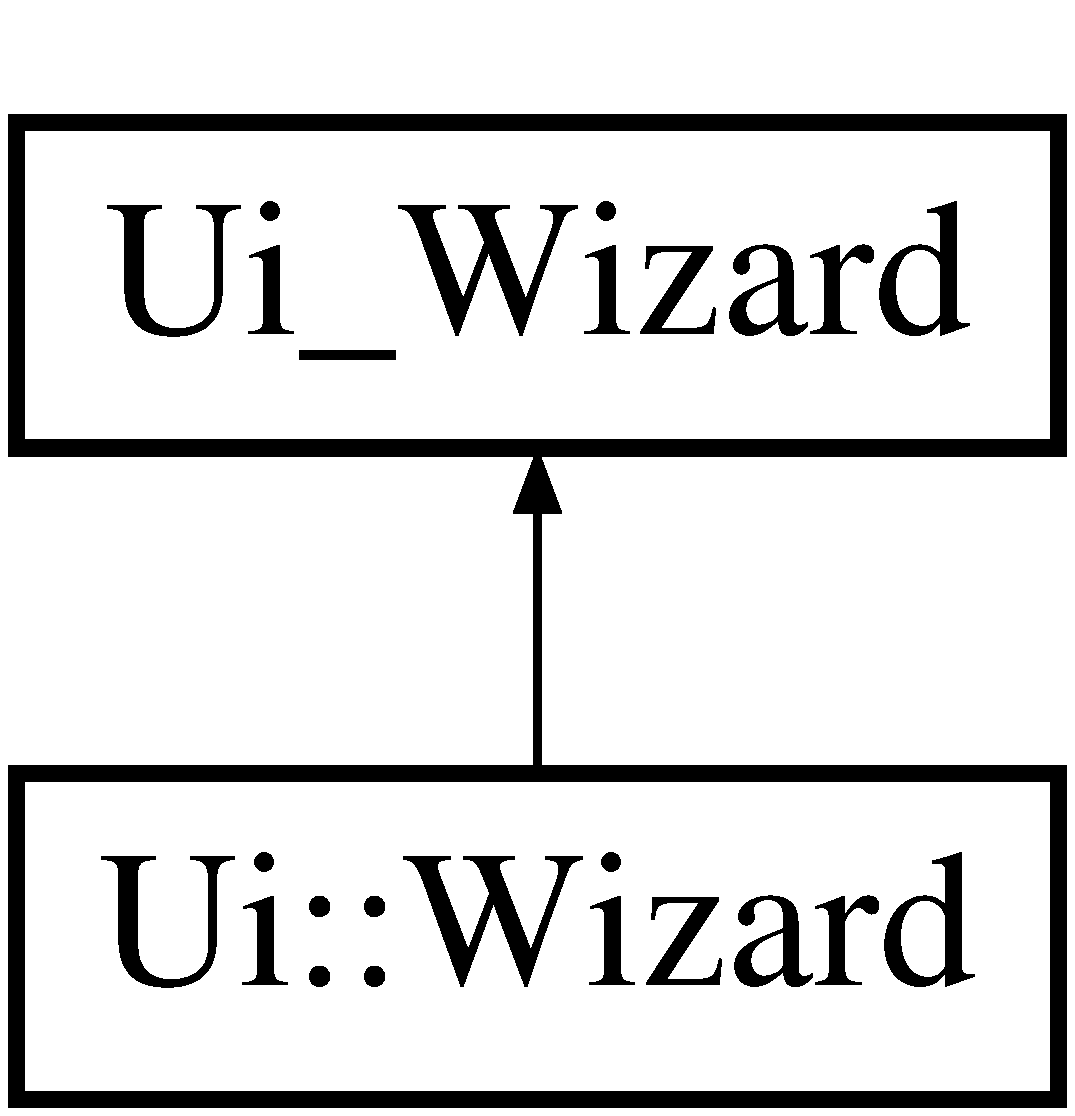
\includegraphics[height=2.000000cm]{class_ui_1_1_wizard}
\end{center}
\end{figure}
\subsection*{Additional Inherited Members}


The documentation for this class was generated from the following file\+:\begin{DoxyCompactItemize}
\item 
ui\+\_\+wizard.\+h\end{DoxyCompactItemize}

\hypertarget{class_wizard}{}\section{Wizard Class Reference}
\label{class_wizard}\index{Wizard@{Wizard}}


Class for the G\+D\+X import wizard.  




{\ttfamily \#include $<$wizard.\+h$>$}

Inheritance diagram for Wizard\+:\begin{figure}[H]
\begin{center}
\leavevmode
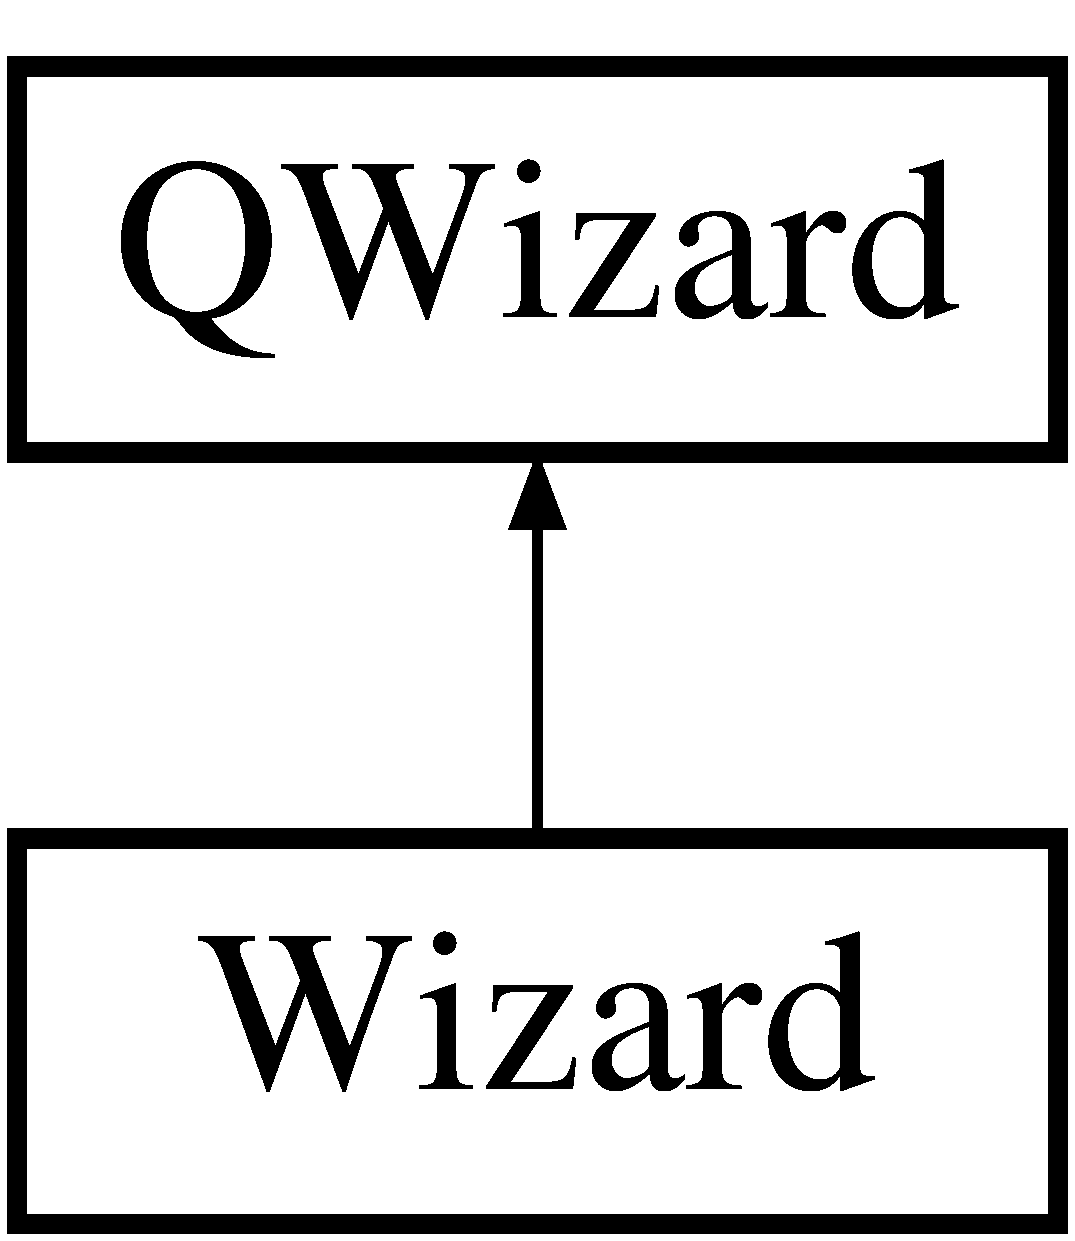
\includegraphics[height=2.000000cm]{class_wizard}
\end{center}
\end{figure}
\subsection*{Signals}
\begin{DoxyCompactItemize}
\item 
\hypertarget{class_wizard_a196e8f8b6c8f346fe869d7f01c2d7ab5}{}void \hyperlink{class_wizard_a196e8f8b6c8f346fe869d7f01c2d7ab5}{create\+Representation} ()\label{class_wizard_a196e8f8b6c8f346fe869d7f01c2d7ab5}

\begin{DoxyCompactList}\small\item\em call \hyperlink{class_main_window_a0b3d1510d0e0ed665daa74d6823e00d6}{Main\+Window\+::create\+Representation()} \end{DoxyCompactList}\item 
\hypertarget{class_wizard_a6f7b8a79c893099e99100bb0c3c67be4}{}void \hyperlink{class_wizard_a6f7b8a79c893099e99100bb0c3c67be4}{add\+Flow} (Q\+String unit1name, Q\+String op1name, Q\+String unit2name, Q\+String op2name, float pr, float cr, float amount)\label{class_wizard_a6f7b8a79c893099e99100bb0c3c67be4}

\begin{DoxyCompactList}\small\item\em call \hyperlink{class_main_window_a645f1cd085c2636dc4eccb320455a6f4}{Main\+Window\+::add\+Flow()} \end{DoxyCompactList}\item 
\hypertarget{class_wizard_a7a17fda2d9854c8461234417c634ec32}{}void \hyperlink{class_wizard_a7a17fda2d9854c8461234417c634ec32}{add\+Task} (Q\+String unit\+Name, Q\+String task\+Name, float start, float end, float amount, Q\+String color=\char`\"{}random\char`\"{})\label{class_wizard_a7a17fda2d9854c8461234417c634ec32}

\begin{DoxyCompactList}\small\item\em call \hyperlink{class_main_window_a2920d5c6c64925cb5f87c7fdac3f54b0}{Main\+Window\+::add\+Task()} \end{DoxyCompactList}\item 
\hypertarget{class_wizard_ae2efd036bcfcaa60c865fed1bec603bd}{}void \hyperlink{class_wizard_ae2efd036bcfcaa60c865fed1bec603bd}{reset} ()\label{class_wizard_ae2efd036bcfcaa60c865fed1bec603bd}

\begin{DoxyCompactList}\small\item\em call \hyperlink{class_main_window_a02076de46e6810174817ebfc6ddd2be5}{Main\+Window\+::reset()} \end{DoxyCompactList}\end{DoxyCompactItemize}
\subsection*{Public Member Functions}
\begin{DoxyCompactItemize}
\item 
\hypertarget{class_wizard_a89dcfb3d0ae3eca49fd820c1e96be8f5}{}{\bfseries Wizard} (Q\+Widget $\ast$parent=0)\label{class_wizard_a89dcfb3d0ae3eca49fd820c1e96be8f5}

\end{DoxyCompactItemize}
\subsection*{Public Attributes}
\begin{DoxyCompactItemize}
\item 
\hypertarget{class_wizard_ab3f30f52640cbbd9ccb5bfd968845a72}{}Q\+String \hyperlink{class_wizard_ab3f30f52640cbbd9ccb5bfd968845a72}{loaded\+File} = \char`\"{}\char`\"{}\label{class_wizard_ab3f30f52640cbbd9ccb5bfd968845a72}

\begin{DoxyCompactList}\small\item\em currently selected gdx file \end{DoxyCompactList}\end{DoxyCompactItemize}
\subsection*{Protected Member Functions}
\begin{DoxyCompactItemize}
\item 
\hypertarget{class_wizard_ad75370785215142ccc6516c5514e26d2}{}bool \hyperlink{class_wizard_ad75370785215142ccc6516c5514e26d2}{validate\+Current\+Page} ()\label{class_wizard_ad75370785215142ccc6516c5514e26d2}

\begin{DoxyCompactList}\small\item\em called at page change \end{DoxyCompactList}\end{DoxyCompactItemize}
\subsection*{Private Slots}
\begin{DoxyCompactItemize}
\item 
\hypertarget{class_wizard_a3e8121fb7eecf94c1c42b9059e0889cd}{}void \hyperlink{class_wizard_a3e8121fb7eecf94c1c42b9059e0889cd}{load\+File\+Clicked} ()\label{class_wizard_a3e8121fb7eecf94c1c42b9059e0889cd}

\begin{DoxyCompactList}\small\item\em load File button clicked \end{DoxyCompactList}\item 
\hypertarget{class_wizard_a0f4d2e63f1dd32a5a824a5aeecc88f43}{}void \hyperlink{class_wizard_a0f4d2e63f1dd32a5a824a5aeecc88f43}{load\+Config\+Clicked} ()\label{class_wizard_a0f4d2e63f1dd32a5a824a5aeecc88f43}

\begin{DoxyCompactList}\small\item\em load Config Button Clicked \end{DoxyCompactList}\item 
\hypertarget{class_wizard_abd795959fb203bacb7f1059d5ee65faf}{}void \hyperlink{class_wizard_abd795959fb203bacb7f1059d5ee65faf}{select\+Sysdir} ()\label{class_wizard_abd795959fb203bacb7f1059d5ee65faf}

\begin{DoxyCompactList}\small\item\em set the G\+A\+M\+S Sysdir if none can be found \end{DoxyCompactList}\item 
\hypertarget{class_wizard_a62b2e1b496cb07ca1f14e4c079470b16}{}void \hyperlink{class_wizard_a62b2e1b496cb07ca1f14e4c079470b16}{save\+Configuration} ()\label{class_wizard_a62b2e1b496cb07ca1f14e4c079470b16}

\begin{DoxyCompactList}\small\item\em save the current configuration \end{DoxyCompactList}\end{DoxyCompactItemize}
\subsection*{Private Member Functions}
\begin{DoxyCompactItemize}
\item 
\hypertarget{class_wizard_aca998aca16aff2aad5a3c14f8b954b6b}{}Q\+String \hyperlink{class_wizard_aca998aca16aff2aad5a3c14f8b954b6b}{get\+Sysdir} ()\label{class_wizard_aca998aca16aff2aad5a3c14f8b954b6b}

\begin{DoxyCompactList}\small\item\em calls \hyperlink{class_wizard_a394f3e7a01cd617aa0759533ab2997ae}{Find\+G\+A\+M\+S()}, returns value as a Q\+String \end{DoxyCompactList}\item 
\hypertarget{class_wizard_a1db1a1c24dc5099792e9ad0d183912e1}{}void \hyperlink{class_wizard_a1db1a1c24dc5099792e9ad0d183912e1}{open\+G\+D\+X} ()\label{class_wizard_a1db1a1c24dc5099792e9ad0d183912e1}

\begin{DoxyCompactList}\small\item\em import the G\+D\+X file \end{DoxyCompactList}\item 
\hypertarget{class_wizard_adfe6a1afa0ef03c25371f32119337644}{}void \hyperlink{class_wizard_adfe6a1afa0ef03c25371f32119337644}{fetch\+Available\+Symbols} ()\label{class_wizard_adfe6a1afa0ef03c25371f32119337644}

\begin{DoxyCompactList}\small\item\em Finds all Symbols in the loaded\+File gdx. \end{DoxyCompactList}\item 
\hypertarget{class_wizard_a7873087523305cb8565a33f68d822cf9}{}void \hyperlink{class_wizard_a7873087523305cb8565a33f68d822cf9}{load\+Symbols\+From\+Config} ()\label{class_wizard_a7873087523305cb8565a33f68d822cf9}

\begin{DoxyCompactList}\small\item\em Loads symbols to use in \hyperlink{class_wizard_a1db1a1c24dc5099792e9ad0d183912e1}{open\+G\+D\+X()} from a previously saved config file. \end{DoxyCompactList}\item 
\hypertarget{class_wizard_a394f3e7a01cd617aa0759533ab2997ae}{}string \hyperlink{class_wizard_a394f3e7a01cd617aa0759533ab2997ae}{Find\+G\+A\+M\+S} ()\label{class_wizard_a394f3e7a01cd617aa0759533ab2997ae}

\begin{DoxyCompactList}\small\item\em Searches for the G\+A\+M\+S Sysdir. \end{DoxyCompactList}\end{DoxyCompactItemize}
\subsection*{Private Attributes}
\begin{DoxyCompactItemize}
\item 
\hypertarget{class_wizard_ad24ade19011c55a41d046fcb77e08e2c}{}\hyperlink{class_ui_1_1_wizard}{Ui\+::\+Wizard} $\ast$ {\bfseries ui}\label{class_wizard_ad24ade19011c55a41d046fcb77e08e2c}

\item 
\hypertarget{class_wizard_a91d00c36482a510a5c84c555b318acbf}{}Q\+String \hyperlink{class_wizard_a91d00c36482a510a5c84c555b318acbf}{loaded\+Config\+File} = \char`\"{}\char`\"{}\label{class_wizard_a91d00c36482a510a5c84c555b318acbf}

\begin{DoxyCompactList}\small\item\em path to the config file \end{DoxyCompactList}\item 
\hypertarget{class_wizard_afb7142f7df6156f74c2e0bb38f48a56a}{}Q\+String \hyperlink{class_wizard_afb7142f7df6156f74c2e0bb38f48a56a}{Sysdir} = \char`\"{}\char`\"{}\label{class_wizard_afb7142f7df6156f74c2e0bb38f48a56a}

\begin{DoxyCompactList}\small\item\em path to the G\+A\+M\+S Sysdir \end{DoxyCompactList}\item 
\hypertarget{class_wizard_a5f8ca2a02c9d656cf4a0f81949c692aa}{}Q\+String\+List $\ast$ \hyperlink{class_wizard_a5f8ca2a02c9d656cf4a0f81949c692aa}{available\+Task\+Symbols}\label{class_wizard_a5f8ca2a02c9d656cf4a0f81949c692aa}

\begin{DoxyCompactList}\small\item\em List of available \hyperlink{struct_task}{Task} symbols. \end{DoxyCompactList}\item 
\hypertarget{class_wizard_af441710077161dca35e55e3498caeb7b}{}Q\+String\+List $\ast$ \hyperlink{class_wizard_af441710077161dca35e55e3498caeb7b}{available\+Flow\+Symbols}\label{class_wizard_af441710077161dca35e55e3498caeb7b}

\begin{DoxyCompactList}\small\item\em List of available \hyperlink{struct_flow}{Flow} symbols. \end{DoxyCompactList}\end{DoxyCompactItemize}


\subsection{Detailed Description}
Class for the G\+D\+X import wizard. 

The documentation for this class was generated from the following files\+:\begin{DoxyCompactItemize}
\item 
wizard.\+h\item 
moc\+\_\+wizard.\+cpp\item 
wizard.\+cpp\end{DoxyCompactItemize}

%--- End generated contents ---

% Index
\backmatter
\newpage
\phantomsection
\clearemptydoublepage
\addcontentsline{toc}{chapter}{Index}
\printindex

\end{document}
